\documentclass{article}
\usepackage{fancyhdr}
\usepackage{ctex}
\usepackage{listings}
\usepackage{graphicx}
\usepackage[a4paper, body={18cm,22cm}]{geometry}
\usepackage{amsmath,amssymb,amstext,wasysym,enumerate,graphicx}
\usepackage{float,abstract,booktabs,indentfirst,amsmath}
\usepackage{array}
\usepackage{booktabs}
\usepackage{multirow}
\usepackage{url}
\usepackage{diagbox}
\renewcommand\arraystretch{1.4}
\usepackage{indentfirst}
\setlength{\parindent}{2em}
\usepackage{enumerate}
\setmonofont{MesloLGS NF}
\usepackage{listings}
\usepackage{xcolor}
\lstset{
    language = [x86masm]Assembler,
    xleftmargin = 3em,xrightmargin = 3em, aboveskip = 1em,
	backgroundcolor = \color{white}, % 背景色
	basicstyle = \small\ttfamily, % 基本样式 + 小号字体
	rulesepcolor= \color{gray}, % 代码块边框颜色
	breaklines = true, % 代码过长则换行
	numbers = left, % 行号在左侧显示
	numberstyle = \small, % 行号字体
    numbersep = -14pt, 
	keywordstyle = \color{blue!50!red!100}, % 关键字颜色
	commentstyle =\color{red!50!green!50!blue!60}, % 注释颜色
	stringstyle = \color{red}, % 字符串颜色
	frame = shadowbox, % 用(带影子效果)方框框住代码块
	showspaces = false, % 不显示空格
	columns = fixed, % 字间距固定
} 
%--------------------页眉--------------------%
\pagestyle{fancy}
\fancyhead[L]{}
\fancyhead[R]{}
\fancyhead[C]{华东师范大学软件工程学院实验报告}
\fancyfoot[C]{-\thepage-}
\renewcommand{\headrulewidth}{1.5pt}
%--------------------标题--------------------%
\begin{document}
\begin{center}
  \LARGE{{\textbf{\heiti 华东师范大学软件工程学院实验报告}}}
  \begin{table}[H]
    \centering
    \begin{tabular}{p{2cm}p{4cm}<{\centering}p{1cm}p{2cm}p{4cm}<{\centering}}
      姓\qquad 名: & 李鹏达 & \quad & 学\qquad 号: & 10225101460            \\ \cline{2-2} \cline{5-5}
      实验编号:    & Lab 02 & \quad & 实验名称:    & Defusing a Binary Bomb
      \\ \cline{2-2} \cline{5-5}
    \end{tabular}
  \end{table}
\end{center}
\rule{\textwidth}{1pt}
%--------------------正文--------------------%
\section{实验目的}
\large
\begin{enumerate}[1)]
  \item 练习汇编代码的阅读
  \item 学习基础的逆向工程和反编译知识
  \item 学习gdb调试工具的使用
\end{enumerate}
\normalsize
\section{实验内容与实验步骤}
\subsection{实验内容}
\large
二进制炸弹是一个由一系列阶段(六个阶段)组成的程序。每个阶段都希望您在标准输入中键入一个特定的字符串。如果您键入正确的字符串,则该阶段将被拆除,炸弹将进入下一阶段。否则,炸弹通过打印“BOOM!!!”爆炸,然后终止。当每个阶段都被拆除时,炸弹就会被拆除。

你在这个实验中的任务是拆除你的炸弹。

\paragraph{1) phase\_1}
阅读反汇编得到的代码中的phase\_1函数,发现其调用了strings\_not\_equal函数,并检测其返回值是否为0。当返回值不为零时,调用函数explode\_bomb引爆炸弹,否则正常进行。

\begin{lstlisting}[title = prase\_1反汇编代码及注释, xleftmargin = 2em,xrightmargin = 2em, aboveskip = 1em, numbers = none, basicstyle=\footnotesize\ttfamily]
346 0000000000400ee0 <phase_1>:
347   400ee0:   48 83 ec 08             sub    $0x8,%rsp                    ; %rsp -= 0x8;
348   400ee4:   be 00 24 40 00          mov    $0x402400,%esi               ; %esi = 0x402400;
349   400ee9:   e8 4a 04 00 00          callq  401338 <strings_not_equal>   ; strings_not_equal(...);
350   400eee:   85 c0                   test   %eax,%eax                    ; if (%eax != 0)
351   400ef0:   74 05                   je     400ef7 <phase_1+0x17>        ;     goto #351;
352   400ef2:   e8 43 05 00 00          callq  40143a <explode_bomb>        ; explode_bomb(...)
353   400ef7:   48 83 c4 08             add    $0x8,%rsp                    ; %rsp += 8;
354   400efb:   c3                      retq                                ; return;
\end{lstlisting}

接下来阅读代码中的strings\_not\_equal函数,不难发现,该函数通过逐字符比较来判断两个字符串是否相同,相同时返回0,不相同时返回1。

在phase\_1中,程序将输入与地址为0x402400的字符串进行了比较,我们可以使用gdb调试工具来展示该地址的字符串。
\begin{lstlisting}[language=bash]
    (gdb) x/s 0x402400
\end{lstlisting}
获得结果如下:
\begin{lstlisting}[language=bash]
    0x402400: "Border relations with Canada have never been better."
\end{lstlisting}


因此答案为“Border relations with Canada have never been better.”
\paragraph{2) phase\_2}


阅读反汇编得到的代码中的phase\_2函数,发现其调用了函数read\_six\_numbers,因此,我们先阅读函数read\_six\_numbers。

\begin{lstlisting}[title = read\_six\_numbers反汇编代码及注释, xleftmargin = 2em,xrightmargin = 2em, aboveskip = 1em, numbers = none, basicstyle=\footnotesize\ttfamily]
804 000000000040145c <read_six_numbers>:
805   40145c:   48 83 ec 18             sub    $0x18,%rsp                       ; %rsp -= 0x18;
806   401460:   48 89 f2                mov    %rsi,%rdx                        ; %rdx = %rsi;
807   401463:   48 8d 4e 04             lea    0x4(%rsi),%rcx                   ; %rcx = %rsi + 0x4;
808   401467:   48 8d 46 14             lea    0x14(%rsi),%rax                  ; %rax = %rsi + 0x14;
809   40146b:   48 89 44 24 08          mov    %rax,0x8(%rsp)                   ; M[%rsp + 0x8] = %rax;
810   401470:   48 8d 46 10             lea    0x10(%rsi),%rax                  ; %rax = %rsi + 0x10;
811   401474:   48 89 04 24             mov    %rax,(%rsp)                      ; M[%rsp] = %rax;
812   401478:   4c 8d 4e 0c             lea    0xc(%rsi),%r9                    ; %r9 = %rsi + 0xc;
813   40147c:   4c 8d 46 08             lea    0x8(%rsi),%r8                    ; %r8 = %rsi + 0x8;
814   401480:   be c3 25 40 00          mov    $0x4025c3,%esi                   ; %esi = 0x4025c3;
815   401485:   b8 00 00 00 00          mov    $0x0,%eax                        ; %eax = 0;
816   40148a:   e8 61 f7 ff ff          callq  400bf0 <__isoc99_sscanf@plt>     ; sscanf(...);
817   40148f:   83 f8 05                cmp    $0x5,%eax                        ; if (%eax > 5)
818   401492:   7f 05                   jg     401499 <read_six_numbers+0x3d>   ;     goto #820;
819   401494:   e8 a1 ff ff ff          callq  40143a <explode_bomb>            ; explode_bomb(...);
820   401499:   48 83 c4 18             add    $0x18,%rsp                       ; %rsp += 0x18;
821   40149d:   c3                      retq                                    ; return;
  \end{lstlisting}

可以发现,在这段代码中,其令\%rdx = \%rsi, \%rcx = \%rsi + 4, \%r8 = \%rsi + 8, \%r9 = \%rsi + 12, M[\%rsp] = \%rsi + 16, M[\%rsp + 8] = \%rsi + 20。可以猜测,其调用sscanf函数将读取的六个数字分别存储到了 \%rdx, \%rcx, \%r8, \%r9, M[\%rsp], M[\%rsp + 8]中, 进而存储到了 $M[\%rsi + k \cdot 4]$中。

接下来阅读phase\_2的反汇编代码。

\begin{lstlisting}[title = phase\_2反汇编代码及注释, xleftmargin = 2em,xrightmargin = 2em, aboveskip = 1em, numbers = none, basicstyle=\footnotesize\ttfamily]
356 0000000000400efc <phase_2>:
357   400efc:   55                      push   %rbp
358   400efd:   53                      push   %rbx
359   400efe:   48 83 ec 28             sub    $0x28,%rsp                   ; %rsp -= 0x28;
360   400f02:   48 89 e6                mov    %rsp,%rsi                    ; %rsi = %rsp;
361   400f05:   e8 52 05 00 00          callq  40145c <read_six_numbers>    ; read_six_numbers(...);
362   400f0a:   83 3c 24 01             cmpl   $0x1,(%rsp)                  ; if (M[%rsp] == 1)
363   400f0e:   74 20                   je     400f30 <phase_2+0x34>        ;     goto #375;
364   400f10:   e8 25 05 00 00          callq  40143a <explode_bomb>        ; explode_bomb(...);
365   400f15:   eb 19                   jmp    400f30 <phase_2+0x34>        ; goto #375;
366   400f17:   8b 43 fc                mov    -0x4(%rbx),%eax              ; %eax = M[%rbx - 4];
367   400f1a:   01 c0                   add    %eax,%eax                    ; %eax += %eax;
368   400f1c: 39 03                   cmp    %eax,(%rbx)                  ; if (%eax == M[%rbx])
369   400f1e:   74 05                   je     400f25 <phase_2+0x29>        ;     goto #371;
370   400f20:   e8 15 05 00 00          callq  40143a <explode_bomb>        ; explode_bomb(...);
371   400f25:   48 83 c3 04             add    $0x4,%rbx                    ; %rbx += 4;
372   400f29:   48 39 eb                cmp    %rbp,%rbx                    ; if (%rbp != %rbx)
373   400f2c:   75 e9                   jne    400f17 <phase_2+0x1b>        ;     goto #366;
374   400f2e:   eb 0c                   jmp    400f3c <phase_2+0x40>        ; goto #378;
375   400f30:   48 8d 5c 24 04          lea    0x4(%rsp),%rbx               ; %rbx = %rsp + 0x4;
376   400f35:   48 8d 6c 24 18          lea    0x18(%rsp),%rbp              ; %rbp = %rsp + 0x18;
377   400f3a:   eb db                   jmp    400f17 <phase_2+0x1b>        ; goto #366;
378   400f3c:   48 83 c4 28             add    $0x28,%rsp                   ; %rsp += 0x28;
379   400f40:   5b                      pop    %rbx
380   400f41:   5d                      pop    %rbp
381   400f42:   c3                      retq
\end{lstlisting}

可以发现,其令\%rsp = \%rsi,因此,读取的六个数字被存储到$M[\%rsp + k\cdot 4]\left( 0 \le k \le 5 \right) $中。根据362行的代码可知,第一个数字为1。阅读代码可以发现,其循环判断后一个数字是否为前一个数字的两倍。因此,可以得知这六个数字为1,2,4,8,16,32。

\paragraph{3) phase\_3}

阅读反汇编得到的代码中的phase\_3函数,发现其令sscanf的第二个参数\%esi = 0x4025cf,使用gdb调试工具得到其内容为“\%d \%d”。

\begin{lstlisting}[language=bash]
    (gdb) x/s 0x4025cf
    0x4025cf:       "%d %d"
  \end{lstlisting}

同时,我们发现程序中使用了间接跳转指令,我们可以使用gdb调试工具来显示跳转表。

\begin{lstlisting}[language=bash]
    (gdb) x/8gx 0x402470
    0x402470:       0x0000000000400f7c      0x0000000000400fb9
    0x402480:       0x0000000000400f83      0x0000000000400f8a
    0x402490:       0x0000000000400f91      0x0000000000400f98
    0x4024a0:       0x0000000000400f9f      0x0000000000400fa6
\end{lstlisting}

我们可以发现,该程序通过sscanf函数读取的两个数字分别存储在$M[\%rsp + 8]$ 和 $M[\%rsp + 0xc]$ 中。根据第一个数字的不同,其通过switch语句进行不同的处理。当其小于8时,分别进行处理,否则引爆炸弹。

\begin{lstlisting}[title = phase\_3反汇编代码及注释, xleftmargin = 2em,xrightmargin = 2em, aboveskip = 1em, numbers = none, basicstyle=\footnotesize\ttfamily]
383 0000000000400f43 <phase_3>:
384   400f43:   48 83 ec 18             sub    $0x18,%rsp                   ; %rsp -= 0x18;
385   400f47:   48 8d 4c 24 0c          lea    0xc(%rsp),%rcx               ; %rcx = %rsp + 0xc;
386   400f4c:   48 8d 54 24 08          lea    0x8(%rsp),%rdx               ; %rdx = %rsp + 0x8;
387   400f51:   be cf 25 40 00          mov    $0x4025cf,%esi               ; %esi = 0x4025cf;
388   400f56:   b8 00 00 00 00          mov    $0x0,%eax                    ; %eax = 0;
389   400f5b:   e8 90 fc ff ff          callq  400bf0 <__isoc99_sscanf@plt> ; sscanf(...)
390   400f60:   83 f8 01                cmp    $0x1,%eax                    ; if (%eax > 1)
391   400f63:   7f 05                   jg     400f6a <phase_3+0x27>        ;     goto #393;
392   400f65:   e8 d0 04 00 00          callq  40143a <explode_bomb>        ; explode_bomb;
393   400f6a:   83 7c 24 08 07          cmpl   $0x7,0x8(%rsp)               ; if (M[%rsp + 0x8] > 7)
394   400f6f:   77 3c                   ja     400fad <phase_3+0x6a>        ;     goto #411;
395   400f71:   8b 44 24 08             mov    0x8(%rsp),%eax               ; %eax = M[%rsp + 0x8];
396   400f75:   ff 24 c5 70 24 40 00    jmpq   *0x402470(,%rax,8)           ; goto 8 * %rax + 0x402470;
397   400f7c:   b8 cf 00 00 00          mov    $0xcf,%eax               ; 0:  %eax = 0xcf;
398   400f81:   eb 3b                   jmp    400fbe <phase_3+0x7b>        ; goto #415;
399   400f83:   b8 c3 02 00 00          mov    $0x2c3,%eax              ; 2:  %eax = 0x2c3;
400   400f88:   eb 34                   jmp    400fbe <phase_3+0x7b>        ; goto #415;
401   400f8a:   b8 00 01 00 00          mov    $0x100,%eax              ; 3:  %eax = 0x100;
402   400f8f:   eb 2d                   jmp    400fbe <phase_3+0x7b>        ; goto #415;
403   400f91:   b8 85 01 00 00          mov    $0x185,%eax              ; 4:  %eax = 0x185;
404   400f96:   eb 26                   jmp    400fbe <phase_3+0x7b>        ; goto #415;
405   400f98:   b8 ce 00 00 00          mov    $0xce,%eax               ; 5:  %eax = 0xce;
406   400f9d:   eb 1f                   jmp    400fbe <phase_3+0x7b>        ; goto #415;
407   400f9f:   b8 aa 02 00 00          mov    $0x2aa,%eax              ; 6:  %eax = 0x2aa;
408   400fa4:   eb 18                   jmp    400fbe <phase_3+0x7b>        ; goto #415;
409   400fa6:   b8 47 01 00 00          mov    $0x147,%eax              ; 7:  %eax = 0x147;
410   400fab:   eb 11                   jmp    400fbe <phase_3+0x7b>        ; goto #415;                       
411   400fad:   e8 88 04 00 00          callq  40143a <explode_bomb>        ; explode_bomb(...);
412   400fb2:   b8 00 00 00 00          mov    $0x0,%eax                    ; %eax = 0;
413   400fb7:   eb 05                   jmp    400fbe <phase_3+0x7b>        ; goto #415;
414   400fb9:   b8 37 01 00 00          mov    $0x137,%eax              ; 1:  %eax = 0x137;
415   400fbe:   3b 44 24 0c             cmp    0xc(%rsp),%eax               ; if (%eax == M[%rsp + 0xc])
416   400fc2:   74 05                   je     400fc9 <phase_3+0x86>        ;     goto #418;
417   400fc4:   e8 71 04 00 00          callq  40143a <explode_bomb>        ; explode_bomb(...);
418   400fc9:   48 83 c4 18             add    $0x18,%rsp                   ; %rsp += 0x18;
419   400fcd:   c3                      retq                                ; return;
\end{lstlisting}

根据代码可以得出,可能的答案有8种,分别是:“0 207”,“1 311”,“2 707”,“3 256”,“4 389”,“5 206”,“6 682”和“7 327”。

\paragraph{4) phase\_4}

阅读反汇编得到的代码中的phase\_4函数,发现其令sscanf的第二个参数\%esi = 0x4025cf,使用gdb调试工具得到其内容为“\%d \%d”。说明其也需读取两个整数。

根据代码可以得出,其读取的第二个整数必须为0,而第一个数必须为小于等于14的数,且当第一个数为参数一,参数二为0,参数三为14时,调用函数func4()时返回值必须为0,否则炸弹将爆炸。

\begin{lstlisting}[title = phase\_4反汇编代码及注释, xleftmargin = 2em,xrightmargin = 2em, aboveskip = 1em, numbers = none, basicstyle=\footnotesize\ttfamily]
445 000000000040100c <phase_4>:
446   40100c:   48 83 ec 18             sub    $0x18,%rsp                   ; %rsp -= 0x18;
447   401010:   48 8d 4c 24 0c          lea    0xc(%rsp),%rcx               ; %rcx = %rsp + 0xc;
448   401015:   48 8d 54 24 08          lea    0x8(%rsp),%rdx               ; %rdx = %rsp + 0x8;
449   40101a:   be cf 25 40 00          mov    $0x4025cf,%esi               ; %esi = 0x4025cf;
450   40101f:   b8 00 00 00 00          mov    $0x0,%eax                    ; %eax = 0;
451   401024:   e8 c7 fb ff ff          callq  400bf0 <__isoc99_sscanf@plt> ; sscanf(...)
452   401029:   83 f8 02                cmp    $0x2,%eax                    ; if (%eax != 2)
453   40102c:   75 07                   jne    401035 <phase_4+0x29>        ;     goto #456;
454   40102e:   83 7c 24 08 0e          cmpl   $0xe,0x8(%rsp)               ; if (M[%rsp + 0x8] <= 0xe)
455   401033:   76 05                   jbe    40103a <phase_4+0x2e>        ;     goto #457;
456   401035:   e8 00 04 00 00          callq  40143a <explode_bomb>        ; explode_bomb(...);
457   40103a:   ba 0e 00 00 00          mov    $0xe,%edx                    ; %edx = 0xe;
458   40103f:   be 00 00 00 00          mov    $0x0,%esi                    ; %rsi = 0;
459   401044:   8b 7c 24 08             mov    0x8(%rsp),%edi               ; %edi = M[%rsp + 0x8];
460   401048:   e8 81 ff ff ff          callq  400fce <func4>               ; func4(%edi, %esi, %edx);
461   40104d:   85 c0                   test   %eax,%eax                    ; if (%eax != 0)
462   40104f:   75 07                   jne    401058 <phase_4+0x4c>        ;     goto #465;
463   401051:   83 7c 24 0c 00          cmpl   $0x0,0xc(%rsp)               ; if (M[%rsp + 0xc] == 0)
464   401056:   74 05                   je     40105d <phase_4+0x51>        ;     goto #466;
465   401058:   e8 dd 03 00 00          callq  40143a <explode_bomb>        ; explode_bomb(...);
466   40105d:   48 83 c4 18             add    $0x18,%rsp                   ; %rsp += 0x18;
467   401061:   c3                      retq                                ; return;
\end{lstlisting}

接下来阅读函数func4。由于其含有递归,较难分析,我们写出其对应的C代码。

\begin{lstlisting}[title = func4反汇编代码及注释, xleftmargin = 2em,xrightmargin = 2em, aboveskip = 1em, numbers = none, basicstyle=\footnotesize\ttfamily]
421 0000000000400fce <func4>:
422   400fce:   48 83 ec 08             sub    $0x8,%rsp                    ; %rsp -= 0x8;
423   400fd2:   89 d0                   mov    %edx,%eax                    ; %eax = %rdx;
424   400fd4:   29 f0                   sub    %esi,%eax                    ; %eax -= %esi;
425   400fd6:   89 c1                   mov    %eax,%ecx                    ; %ecx = %eax;
426   400fd8:   c1 e9 1f                shr    $0x1f,%ecx                   ; %ecx >>=(H) 0x1f;
427   400fdb:   01 c8                   add    %ecx,%eax                    ; %eax += %ecx;
428   400fdd:   d1 f8                   sar    %eax                         ; %eax >>= 1;
429   400fdf:   8d 0c 30                lea    (%rax,%rsi,1),%ecx           ; %ecx = %rax + %rsi;
430   400fe2:   39 f9                   cmp    %edi,%ecx                    ; if (%ecx <= %edi)
431   400fe4:   7e 0c                   jle    400ff2 <func4+0x24>          ;     goto #436;
432   400fe6:   8d 51 ff                lea    -0x1(%rcx),%edx              ; %edx = %rcx - 1;
433   400fe9:   e8 e0 ff ff ff          callq  400fce <func4>               ; func4(%rdi, %rsi, %rdx);
434   400fee:   01 c0                   add    %eax,%eax                    ; %eax += %eax;
435   400ff0:   eb 15                   jmp    401007 <func4+0x39>          ; goto #442;
436   400ff2:   b8 00 00 00 00          mov    $0x0,%eax                    ; %eax = 0;
437   400ff7:   39 f9                   cmp    %edi,%ecx                    ; if (%ecx >= %edi)
438   400ff9:   7d 0c                   jge    401007 <func4+0x39>          ;     goto #442;
439   400ffb:   8d 71 01                lea    0x1(%rcx),%esi               ; %esi = %rcx + 1;
440   400ffe:   e8 cb ff ff ff          callq  400fce <func4>               ; func4(%rdi, %rsi, %rdx);
441   401003:   8d 44 00 01             lea    0x1(%rax,%rax,1),%eax        ; %eax = 2 * %rax + 1;
442   401007:   48 83 c4 08             add    $0x8,%rsp                    ; %rsp += 8;
443   40100b:   c3                      retq                                ; return %eax;
\end{lstlisting}

\begin{lstlisting}[title = func4对应的C代码, xleftmargin = 2em,xrightmargin = 2em, aboveskip = 1em, numbers = left, language=c]
    int func4(int a, int b, int c) {
    // a in %rdi, b in %rsi, c in %rdx
        int d = (c - b) / 2;
        int e = (c + b) / 2;
        if (e <= a) {
            d = 0;
            if (e >= a) {
                return d;
            } else {
                d = func4(a, e + 1, c);
                d = 2 * d + 1;
                return d;
            }
        } else {
            d = func4(a, b, e - 1);
            d = 2 * d;
            return d;
        }
    }
\end{lstlisting}

对这份C代码进行测试,可以得知:0,1,3和7是满足返回值为0的参数a。

因此,满足要求的答案为:“0 0”,“1 0”,“3 0”和“7 0”。

\paragraph{5) phase\_5}

阅读反汇编得到的代码中的phase\_5函数,可以发现,其读取了一个字符串,并判断了字符串的长度,在字符串长度不等于6时引爆炸弹。

并且,其通过循环,将读取的字符串中的每一个字符进行了处理。设字符为$c$,其将$c\,\&\,0xf$的结果作为下标,令$M[\%rsp + 0x10 + i]=M[c\&0xf + 0x4024b0]$。

接着,它判断了M[\%rsp + 10]处的字符串与0x40245e处的字符串是否相同。如果不同,则引爆炸弹。

\begin{lstlisting}[title = phase\_5对应的反汇编代码及注释, xleftmargin = 2em,xrightmargin = 2em, aboveskip = 1em, numbers = none, basicstyle=\footnotesize\ttfamily]
469 0000000000401062 <phase_5>:
470   401062:   53                      push   %rbx
471   401063:   48 83 ec 20             sub    $0x20,%rsp                   ; %rsp -= 0x20;
472   401067:   48 89 fb                mov    %rdi,%rbx                    ; %rbx = %rdi;
473   40106a:   64 48 8b 04 25 28 00    mov    %fs:0x28,%rax                ; %rax = 0x28;
474   401071:   00 00
475   401073:   48 89 44 24 18          mov    %rax,0x18(%rsp)              ; M[%rsp + 0x18] = %rax;
476   401078:   31 c0                   xor    %eax,%eax                    ; %eax ^= %eax;
477   40107a:   e8 9c 02 00 00          callq  40131b <string_length>       ; string_length(%rdi);
478   40107f:   83 f8 06                cmp    $0x6,%eax                    ; if (%eax == 6)
479   401082:   74 4e                   je     4010d2 <phase_5+0x70>        ;     goto #500;
480   401084:   e8 b1 03 00 00          callq  40143a <explode_bomb>        ; explode_bomb(...);
481   401089:   eb 47                   jmp    4010d2 <phase_5+0x70>        ; goto #500;
482   40108b:   0f b6 0c 03             movzbl (%rbx,%rax,1),%ecx           ; %ecx = %rbx + %rax;
483   40108f:   88 0c 24                mov    %cl,(%rsp)                   ; M[%rsp] = %cl;
484   401092:   48 8b 14 24             mov    (%rsp),%rdx                  ; %rdx = M[%rsp];
485   401096:   83 e2 0f                and    $0xf,%edx                    ; %edx &= 0xf;
486   401099:   0f b6 92 b0 24 40 00    movzbl 0x4024b0(%rdx),%edx          ; %edx = M[%rdx + 0x4024b0];
487   4010a0:   88 54 04 10             mov    %dl,0x10(%rsp,%rax,1)        ; M[%rsp + %rax + 0x10] = %dl;
488   4010a4:   48 83 c0 01             add    $0x1,%rax                    ; %rax++;
489   4010a8:   48 83 f8 06             cmp    $0x6,%rax                    ; if (%rax != 0x6)
490   4010ac:   75 dd                   jne    40108b <phase_5+0x29>        ;     goto #482;
491   4010ae:   c6 44 24 16 00          movb   $0x0,0x16(%rsp)              ; M[%rsp + 0x16] = 0;
492   4010b3:   be 5e 24 40 00          mov    $0x40245e,%esi               ; %esi = 0x40245e;
493   4010b8:   48 8d 7c 24 10          lea    0x10(%rsp),%rdi              ; %rdi = %rsp + 0x10;
494   4010bd:   e8 76 02 00 00          callq  401338 <strings_not_equal>   ; strings_not_equal(%rdi, %rsi);
495   4010c2:   85 c0                   test   %eax,%eax                    ; if (%eax == 0)
496   4010c4:   74 13                   je     4010d9 <phase_5+0x77>        ;     goto #502;
497   4010c6:   e8 6f 03 00 00          callq  40143a <explode_bomb>        ; explode_bomb(...);
498   4010cb:   0f 1f 44 00 00          nopl   0x0(%rax,%rax,1)             ; ???
499   4010d0:   eb 07                   jmp    4010d9 <phase_5+0x77>        ; goto #502;
500   4010d2:   b8 00 00 00 00          mov    $0x0,%eax                    ; %eax = 0;
501   4010d7:   eb b2                   jmp    40108b <phase_5+0x29>        ; goto #482;
502   4010d9:   48 8b 44 24 18          mov    0x18(%rsp),%rax              ; %rax = M[%rsp + 0x18];
503   4010de:   64 48 33 04 25 28 00    xor    %fs:0x28,%rax                ; %rax ^= 0x28;
504   4010e5:   00 00
505   4010e7:   74 05                   je     4010ee <phase_5+0x8c>        ; goto #507;
506   4010e9:   e8 42 fa ff ff          callq  400b30 <__stack_chk_fail@plt>;
507   4010ee:   48 83 c4 20             add    $0x20,%rsp                   ; %rsp += 0x20;
508   4010f2:   5b                      pop    %rbx
509   4010f3:   c3                      retq
  \end{lstlisting}

使用gdb调试工具可以得到0x4024b0和0x40245e处的字符串内容。

\begin{lstlisting}[language=bash]
    (gdb) x/s 0x40245e
    0x40245e:       "flyers"
    (gdb) x/s 0x4024b0
    0x4024b0 <array.3449>:  "maduiersnfotvbylSo you think you can stop the bomb with ctrl-c, do you?"
\end{lstlisting}

为了找出满足条件的字符串,我们可以使用C++编程解决。

\begin{lstlisting}[language=C++, title=解决此问题的C++代码]
    #include <iostream>
    #include <vector>
    int main() {
        std::string tar = "flyers";
        std::string s = "maduiersnfotvbylSo you think you can stop the bomb with ctrl-c, do you?";
        std::vector<std::vector<char>> ans(6, std::vector<char>(0));
        for (int i = 0; i < 6; i++) {
            for (int j = 32; j < 127; j++) {
                char k = j & 0xf;
                if (k < s.size() && s[k] == tar[i]) {
                    ans[i].push_back(j);
                }
            }
        }
        for (auto i : ans) {
            for (auto j : i) {
                std::cout << j << ' ';
            }
            std::cout << std::endl;
        }
    }
  \end{lstlisting}

答案如下表所示,共有38880种组合。

\begin{table}[!htbp]
  \centering
  \begin{tabular}{|c|c|c|c|c|c|c|}
    \hline
    \diagbox{位置(下标)}{可能的字符} & 1  & 2 & 3 & 4    & 5 & 6    \\
    \hline
    0                                  & )  & 9 & I & Y    & i & y    \\
    \hline
    1                                  & /  & ? & O & \_   & o & 无   \\
    \hline
    2                                  & .  & > & N & $\^$ & n & $\~$ \\
    \hline
    3                                  & \% & 5 & E & U    & e & u    \\
    \hline
    4                                  & \& & 6 & F & V    & f & v    \\
    \hline
    5                                  & '  & 7 & G & W    & g & w    \\
    \hline
  \end{tabular}
\end{table}

\paragraph{6) phase\_6}
阅读反汇编得到的代码中的phase\_6函数,可以发现其首先读取了六个数字。

接着,它判断了读取到的第一个数字与6的大小关系,如果第一个数字不满足小于等于6,则引爆炸弹。

接下来,其使用\%ebx和\%r12d作为计数器,循环检查了剩余五个数字是否与 \%rbp相同,如果与\%rbp相同,则引爆炸弹。而在循环中,\%rbp依次被赋给前五个数字的值,即这段代码检查了输入的数字中是否存在相同的数字,如果存在,则引爆炸弹。同时,循环中也再次检查了每一个数字是否满足小于等于6,如果不满足,则引爆炸弹。

接着,程序通过循环,令$M[\%rsp + 4 \cdot k] = 7 - M[\%rsp + 4 \cdot k]$。即用7分别减去了读入的6个数字。

此时,代码中出现了内存地址0x6032d0,可以用gdb调试器列出其值,经过尝试,可以发现它是一个链表。

\begin{lstlisting}[language=bash, xleftmargin=2em, xrightmargin=2em]
    (gdb) x/24x 0x6032d0
    0x6032d0 <node1>:       0x0000014c      0x00000001      0x006032e0      0x00000000
    0x6032e0 <node2>:       0x000000a8      0x00000002      0x006032f0      0x00000000
    0x6032f0 <node3>:       0x0000039c      0x00000003      0x00603300      0x00000000
    0x603300 <node4>:       0x000002b3      0x00000004      0x00603310      0x00000000
    0x603310 <node5>:       0x000001dd      0x00000005      0x00603320      0x00000000
    0x603320 <node6>:       0x000001bb      0x00000006      0x00000000      0x00000000
\end{lstlisting}

设经过操作后的数为$x_k$,地址为$\%rsp + 4\cdot k$,若$x_k \le 1$(即操作前$\ge 6$),则令$M[\%rsp + 0x20 + 2 \cdot k] = 0x6032d0$,即链表的第一个节点。实际上,由于每一个读入的数字都是不重复且小于等于6的,只有在其等于6时,即操作后$x_k=1$时,才能满足这个条件。若$x_k>1$,即操作前$<6$,则先通过循环,找到链表中第$x_k$个节点$nodex_k$,再令$M[\%rsp + 0x20 + 2 \cdot k] = \&nodex_k$。简要来说,这段代码完成了令$M[\%rsp + 0x20 + 8\cdot k] = \&nodex_k$的操作。

接下来,代码通过循环重新链接了链表的六个节点。重新链接后的顺序与其陈列在$M[\%rsp + 0x20]$处的顺序相同。

最后,程序通过循环,判断重新链接后的链表中是否满足前一个数大于后一个数。只要有一个不满足,炸弹将爆炸。

\begin{lstlisting}[title = phase\_6对应的反汇编代码及注释, xleftmargin = 2em,xrightmargin = 2em, aboveskip = 1em, numbers = none, basicstyle=\footnotesize\ttfamily]
511 00000000004010f4 <phase_6>:
512   4010f4:   41 56                   push   %r14
513   4010f6:   41 55                   push   %r13
514   4010f8:   41 54                   push   %r12
515   4010fa:   55                      push   %rbp
516   4010fb:   53                      push   %rbx
517   4010fc:   48 83 ec 50             sub    $0x50,%rsp                   ; %rsp -= 0x50;
518   401100:   49 89 e5                mov    %rsp,%r13                    ; %r13 = %rsp;
519   401103:   48 89 e6                mov    %rsp,%rsi                    ; %rsi = %rsp;
520   401106:   e8 51 03 00 00          callq  40145c <read_six_numbers>    ; read_six_numbers(...);
521   40110b:   49 89 e6                mov    %rsp,%r14                    ; %r14 = %rsp;
522   40110e:   41 bc 00 00 00 00       mov    $0x0,%r12d                   ; %r12d = 0;
523   401114:   4c 89 ed                mov    %r13,%rbp                    ; %rbp = %r13;
524   401117:   41 8b 45 00             mov    0x0(%r13),%eax               ; %eax = M[%r13];
525   40111b:   83 e8 01                sub    $0x1,%eax                    ; %eax--;
526   40111e:   83 f8 05                cmp    $0x5,%eax                    ; if (%eax <= 5)
527   401121:   76 05                   jbe    401128 <phase_6+0x34>        ;     goto #529;
528   401123:   e8 12 03 00 00          callq  40143a <explode_bomb>        ; explode_bomb(...);
529   401128:   41 83 c4 01             add    $0x1,%r12d                   ; %r12d++;
530   40112c:   41 83 fc 06             cmp    $0x6,%r12d                   ; if (%r12d == 6)
531   401130:   74 21                   je     401153 <phase_6+0x5f>        ;     goto #543;
532   401132:   44 89 e3                mov    %r12d,%ebx                   ; %ebx = %r12d;
533   401135:   48 63 c3                movslq %ebx,%rax                    ; %rax = %ebx;
534   401138:   8b 04 84                mov    (%rsp,%rax,4),%eax           ; %eax = M[%rsp + %eax * 4];
535   40113b:   39 45 00                cmp    %eax,0x0(%rbp)               ; if (M[%rbp] != %eax)
536   40113e:   75 05                   jne    401145 <phase_6+0x51>        ;     goto #538;
537   401140:   e8 f5 02 00 00          callq  40143a <explode_bomb>        ; explode_bomb(...);
538   401145:   83 c3 01                add    $0x1,%ebx                    ; %ebx++;
539   401148:   83 fb 05                cmp    $0x5,%ebx                    ; if (%ebx <= 5)
540   40114b:   7e e8                   jle    401135 <phase_6+0x41>        ;     goto #533;
541   40114d:   49 83 c5 04             add    $0x4,%r13                    ; %r13 += 4;
542   401151:   eb c1                   jmp    401114 <phase_6+0x20>        ; goto #523;
543   401153:   48 8d 74 24 18          lea    0x18(%rsp),%rsi              ; %rsi = %rsp + 0x18;
544   401158:   4c 89 f0                mov    %r14,%rax                    ; %rax = %r14;
545   40115b:   b9 07 00 00 00          mov    $0x7,%ecx                    ; %ecx = 0x7;
546   401160:   89 ca                   mov    %ecx,%edx                    ; %edx = %ecx;
547   401162:   2b 10                   sub    (%rax),%edx                  ; %edx -= M[%rax];
548   401164:   89 10                   mov    %edx,(%rax)                  ; M[%rax] = %edx;
549   401166:   48 83 c0 04             add    $0x4,%rax                    ; %rax += 4;
550   40116a:   48 39 f0                cmp    %rsi,%rax                    ; if (%rax != %rsi)
551   40116d:   75 f1                   jne    401160 <phase_6+0x6c>        ;     goto #546;
552   40116f:   be 00 00 00 00          mov    $0x0,%esi                    ; %esi = 0;
553   401174:   eb 21                   jmp    401197 <phase_6+0xa3>        ; goto #564;
554   401176:   48 8b 52 08             mov    0x8(%rdx),%rdx               ; %rdx = M[%rdx + 8];
555   40117a:   83 c0 01                add    $0x1,%eax                    ; %eax++;
556   40117d:   39 c8                   cmp    %ecx,%eax                    ; if (%eax != %ecx)
557   40117f:   75 f5                   jne    401176 <phase_6+0x82>        ;     goto #554;
558   401181:   eb 05                   jmp    401188 <phase_6+0x94>        ; goto #560;
559   401183:   ba d0 32 60 00          mov    $0x6032d0,%edx               ; %edx = 0x6032d0;
560   401188:   48 89 54 74 20          mov    %rdx,0x20(%rsp,%rsi,2)       ; M[%rsp + %rsi * 2 + 0x20] = %rdx;
561   40118d:   48 83 c6 04             add    $0x4,%rsi                    ; %rsi += 4;
562   401191:   48 83 fe 18             cmp    $0x18,%rsi                   ; if (%rsi == 0x18)
563   401195:   74 14                   je     4011ab <phase_6+0xb7>        ;     goto #570;
564   401197:   8b 0c 34                mov    (%rsp,%rsi,1),%ecx           ; %ecx = M[%rsp + %rsi];
565   40119a:   83 f9 01                cmp    $0x1,%ecx                    ; if (%ecx <= 1)
566   40119d:   7e e4                   jle    401183 <phase_6+0x8f>        ;     goto #559;
567   40119f:   b8 01 00 00 00          mov    $0x1,%eax                    ; %eax = 1;
568   4011a4:   ba d0 32 60 00          mov    $0x6032d0,%edx               ; %edx = 0x6032d0;
569   4011a9:   eb cb                   jmp    401176 <phase_6+0x82>        ; goto #554;
570   4011ab:   48 8b 5c 24 20          mov    0x20(%rsp),%rbx              ; %rbx = M[%rsp + 0x20];
571   4011b0:   48 8d 44 24 28          lea    0x28(%rsp),%rax              ; %rax = %rsp + 0x28;
572   4011b5:   48 8d 74 24 50          lea    0x50(%rsp),%rsi              ; %rsi = %rsp + 0x50;
573   4011ba:   48 89 d9                mov    %rbx,%rcx                    ; %rcx = %rbx;
574   4011bd:   48 8b 10                mov    (%rax),%rdx                  ; %rdx = M[%rax];
575   4011c0:   48 89 51 08             mov    %rdx,0x8(%rcx)               ; M[%rcx + 0x8] = %rdx;
576   4011c4:   48 83 c0 08             add    $0x8,%rax                    ; %rax += 8;
577   4011c8:   48 39 f0                cmp    %rsi,%rax                    ; if (%rax == %rsi)
578   4011cb:   74 05                   je     4011d2 <phase_6+0xde>        ;     goto #581;
579   4011cd:   48 89 d1                mov    %rdx,%rcx                    ; %rcx = %rdx;
580   4011d0:   eb eb                   jmp    4011bd <phase_6+0xc9>        ; goto #574;
581   4011d2:   48 c7 42 08 00 00 00    movq   $0x0,0x8(%rdx)               ; M[%rdx + 8] = 0;
582   4011d9:   00
583   4011da:   bd 05 00 00 00          mov    $0x5,%ebp                    ; %ebp = 5;
584   4011df:   48 8b 43 08             mov    0x8(%rbx),%rax               ; %rax = M[%rbx + 8];
585   4011e3:   8b 00                   mov    (%rax),%eax                  ; %eax = M[%rax];
586   4011e5:   39 03                   cmp    %eax,(%rbx)                  ; if (M[%rbx] >= %eax)
587   4011e7:   7d 05                   jge    4011ee <phase_6+0xfa>        ;     goto #589;
588   4011e9:   e8 4c 02 00 00          callq  40143a <explode_bomb>        ; explode_bomb(...);
589   4011ee:   48 8b 5b 08             mov    0x8(%rbx),%rbx               ; %rbx = M[%rbx + 8];
590   4011f2:   83 ed 01                sub    $0x1,%ebp                    ; %ebp--;
591   4011f5:   75 e8                   jne    4011df <phase_6+0xeb>        ; goto #584;
592   4011f7:   48 83 c4 50             add    $0x50,%rsp                   ; %rsp += 0x50;
593   4011fb:   5b                      pop    %rbx
594   4011fc:   5d                      pop    %rbp
595   4011fd:   41 5c                   pop    %r12
596   4011ff:   41 5d                   pop    %r13
597   401201:   41 5e                   pop    %r14
598   401203:   c3                      retq
  \end{lstlisting}

通过gdb调试工具可以得知,原链表中的值为322,168,924,691,477,443。
\begin{lstlisting}[language=bash]
    (gdb) x/24d 0x6032d0
    0x6032d0 <node1>:       332     1       6304480 0
    0x6032e0 <node2>:       168     2       6304496 0
    0x6032f0 <node3>:       924     3       6304512 0
    0x603300 <node4>:       691     4       6304528 0
    0x603310 <node5>:       477     5       6304544 0
    0x603320 <node6>:       443     6       0       0
  \end{lstlisting}

其中,节点按从大到小依次排序为3,4,5,6,1,2。用7减去后为4,3,2,1,6,5。

即答案为“4 3 2 1 6 5”。

\paragraph{7) secret\_phase}首先我们需要找到secret\_phase的入口。

在文件中搜索,可以发现在phase\_defused函数中调用了secret\_phase。可以发现,在这个函数中,其调用了sscanf函数以0x603870作为源,0x402619作为格式读取了内容,当且仅当$num\_input\_strings = 6$且读取到的内容为三个且读取到的第三个内容与0x402622处的字符串相同时,secret\_phase才会被调用。

\begin{lstlisting}[title = phase\_defused对应的反汇编代码, xleftmargin = 0.5em,xrightmargin = 0.5em, aboveskip = 1em, numbers = none, basicstyle=\footnotesize\ttfamily]
892 00000000004015c4 <phase_defused>:
893   4015c4:   48 83 ec 78             sub    $0x78,%rsp
894   4015c8:   64 48 8b 04 25 28 00    mov    %fs:0x28,%rax
895   4015cf:   00 00
896   4015d1:   48 89 44 24 68          mov    %rax,0x68(%rsp)
897   4015d6:   31 c0                   xor    %eax,%eax
898   4015d8:   83 3d 81 21 20 00 06    cmpl   $0x6,0x202181(%rip)        # 603760 <num_input_strings>
899   4015df:   75 5e                   jne    40163f <phase_defused+0x7b>
900   4015e1:   4c 8d 44 24 10          lea    0x10(%rsp),%r8
901   4015e6:   48 8d 4c 24 0c          lea    0xc(%rsp),%rcx
902   4015eb:   48 8d 54 24 08          lea    0x8(%rsp),%rdx
903   4015f0:   be 19 26 40 00          mov    $0x402619,%esi
904   4015f5:   bf 70 38 60 00          mov    $0x603870,%edi
905   4015fa:   e8 f1 f5 ff ff          callq  400bf0 <__isoc99_sscanf@plt>
906   4015ff:   83 f8 03                cmp    $0x3,%eax
907   401602:   75 31                   jne    401635 <phase_defused+0x71>
908   401604:   be 22 26 40 00          mov    $0x402622,%esi
909   401609:   48 8d 7c 24 10          lea    0x10(%rsp),%rdi
910   40160e:   e8 25 fd ff ff          callq  401338 <strings_not_equal>
911   401613:   85 c0                   test   %eax,%eax
912   401615:   75 1e                   jne    401635 <phase_defused+0x71>
913   401617:   bf f8 24 40 00          mov    $0x4024f8,%edi
914   40161c:   e8 ef f4 ff ff          callq  400b10 <puts@plt>
915   401621:   bf 20 25 40 00          mov    $0x402520,%edi
916   401626:   e8 e5 f4 ff ff          callq  400b10 <puts@plt>
917   40162b:   b8 00 00 00 00          mov    $0x0,%eax
918   401630:   e8 0d fc ff ff          callq  401242 <secret_phase>                                           
919   401635:   bf 58 25 40 00          mov    $0x402558,%edi
920   40163a:   e8 d1 f4 ff ff          callq  400b10 <puts@plt>
921   40163f:   48 8b 44 24 68          mov    0x68(%rsp),%rax
922   401644:   64 48 33 04 25 28 00    xor    %fs:0x28,%rax
923   40164b:   00 00
924   40164d:   74 05                   je     401654 <phase_defused+0x90>
925   40164f:   e8 dc f4 ff ff          callq  400b30 <__stack_chk_fail@plt>
926   401654:   48 83 c4 78             add    $0x78,%rsp
927   401658:   c3                      retq
928   401659:   90                      nop
929   40165a:   90                      nop
930   40165b:   90                      nop
931   40165c:   90                      nop
932   40165d:   90                      nop
933   40165e:   90                      nop
934   40165f:   90                      nop
  \end{lstlisting}

使用gdb调试工具打印这些地址所对应的内容。

\begin{lstlisting}[language=bash]
    (gdb) x/s 0x603870
    0x603870 <input_strings+240>:   ""
    (gdb) x/s 0x402619
    0x402619:       "%d %d %s"
    (gdb) x/s 0x402622
    0x402622:       "DrEvil"
\end{lstlisting}

可以发现,0x603870所对应的内容是我们之前输入的内容的一部分,因此我们使用调试工具,在完成前6个phase后再查看此地址的内容。

\begin{lstlisting}[language=bash, commentstyle=\color{black}]
    (gdb) b phase_defused if ((int)num_input_strings == 6)
    Breakpoint 1 at 0x4015c4
    (gdb) r
    Starting program: /home/pdli/Desktop/lab2/bomb/bomb
    Welcome to my fiendish little bomb. You have 6 phases with
    which to blow yourself up. Have a nice day!
    Border relations with Canada have never been better.
    Phase 1 defused. How about the next one?
    1 2 4 8 16 32
#   That's number 2.  Keep going!
    7 327
    Halfway there!
    0 0
    So you got that one.  Try this one.
    9?>567
    Good work!  On to the next...
    4 3 2 1 6 5

    Breakpoint 1, 0x00000000004015c4 in phase_defused ()
    (gdb) x/s 0x603870
    0x603870 <input_strings+240>:   "0 0"
\end{lstlisting}

可以发现,其对应的是在phase\_4中我们输入的字符串。因此,若想要进入secret\_phase,我们需要在phase\_4的答案后加上“DrEvil”。

接下来,我们分析secret\_phase的内容。

\begin{lstlisting}[title = secret\_phase对应的反汇编代码及注释, xleftmargin = 2em,xrightmargin = 2em, aboveskip = 1em, numbers = none, basicstyle=\footnotesize\ttfamily]
622 0000000000401242 <secret_phase>:
623   401242:   53                      push   %rbx
624   401243:   e8 56 02 00 00          callq  40149e <read_line>           ; read_line(...);
625   401248:   ba 0a 00 00 00          mov    $0xa,%edx                    ; %edx = 0xa;
626   40124d:   be 00 00 00 00          mov    $0x0,%esi                    ; %esi = 0x0;
627   401252:   48 89 c7                mov    %rax,%rdi                    ; %rdi = %rax;
628   401255:   e8 76 f9 ff ff          callq  400bd0 <strtol@plt>          ; strtol(...);
629   40125a:   48 89 c3                mov    %rax,%rbx                    ; %rbx = %rax;
630   40125d:   8d 40 ff                lea    -0x1(%rax),%eax              ; %eax--;
631   401260:   3d e8 03 00 00          cmp    $0x3e8,%eax                  ; if (%eax <= 0x3e8)
632   401265:   76 05                   jbe    40126c <secret_phase+0x2a>   ;     goto #634;
633   401267:   e8 ce 01 00 00          callq  40143a <explode_bomb>        ; explode_bomb(...);
634   40126c:   89 de                   mov    %ebx,%esi                    ; %esi = %ebx;
635   40126e:   bf f0 30 60 00          mov    $0x6030f0,%edi               ; %edi = 0x6030f0;
636   401273:   e8 8c ff ff ff          callq  401204 <fun7>                ; fun7(%rdi, %rsi);
637   401278:   83 f8 02                cmp    $0x2,%eax                    ; if (%eax == 2)
638   40127b:   74 05                   je     401282 <secret_phase+0x40>   ;     goto #640;
639   40127d:   e8 b8 01 00 00          callq  40143a <explode_bomb>        ; explode_bomb(...);
640   401282:   bf 38 24 40 00          mov    $0x402438,%edi               ; %edi = 0x402438;
641   401287:   e8 84 f8 ff ff          callq  400b10 <puts@plt>            ; puts(%rdi);
642   40128c:   e8 33 03 00 00          callq  4015c4 <phase_defused>       ; phase_defused(...);
643   401291:   5b                      pop    %rbx
644   401292:   c3                      retq
645   401293:   90                      nop
646   401294:   90                      nop
647   401295:   90                      nop
648   401296:   90                      nop                                                               
649   401297:   90                      nop
650   401298:   90                      nop
651   401299:   90                      nop
652   40129a:   90                      nop
653   40129b:   90                      nop
654   40129c:   90                      nop
655   40129d:   90                      nop
656   40129e:   90                      nop
657   40129f:   90                      nop
  \end{lstlisting}

可以发现其与地址0x6030f0的内容有关,我们可以使用gdb调试工具尝试获取该地址的内容,经过尝试,可以发现此处存储的数据结构是一个二叉树。
\begin{lstlisting}[language=bash, commentstyle=\color{black}]
    0x6030f0 <n1>:  0x0000000000000024      0x0000000000603110
    0x603100 <n1+16>:       0x0000000000603130      0x0000000000000000
    0x603110 <n21>: 0x0000000000000008      0x0000000000603190
    0x603120 <n21+16>:      0x0000000000603150      0x0000000000000000
    0x603130 <n22>: 0x0000000000000032      0x0000000000603170
    0x603140 <n22+16>:      0x00000000006031b0      0x0000000000000000
    0x603150 <n32>: 0x0000000000000016      0x0000000000603270
    0x603160 <n32+16>:      0x0000000000603230      0x0000000000000000
    0x603170 <n33>: 0x000000000000002d      0x00000000006031d0
    0x603180 <n33+16>:      0x0000000000603290      0x0000000000000000
    0x603190 <n31>: 0x0000000000000006      0x00000000006031f0
    0x6031a0 <n31+16>:      0x0000000000603250      0x0000000000000000
    0x6031b0 <n34>: 0x000000000000006b      0x0000000000603210
    0x6031c0 <n34+16>:      0x00000000006032b0      0x0000000000000000
    0x6031d0 <n45>: 0x0000000000000028      0x0000000000000000
    0x6031e0 <n45+16>:      0x0000000000000000      0x0000000000000000
    0x6031f0 <n41>: 0x0000000000000001      0x0000000000000000
    0x603200 <n41+16>:      0x0000000000000000      0x0000000000000000
    0x603210 <n47>: 0x0000000000000063      0x0000000000000000
    0x603220 <n47+16>:      0x0000000000000000      0x0000000000000000
    0x603230 <n44>: 0x0000000000000023      0x0000000000000000
    0x603240 <n44+16>:      0x0000000000000000      0x0000000000000000
    0x603250 <n42>: 0x0000000000000007      0x0000000000000000
    0x603260 <n42+16>:      0x0000000000000000      0x0000000000000000
    0x603270 <n43>: 0x0000000000000014      0x0000000000000000
    0x603280 <n43+16>:      0x0000000000000000      0x0000000000000000
    0x603290 <n46>: 0x000000000000002f      0x0000000000000000
    0x6032a0 <n46+16>:      0x0000000000000000      0x0000000000000000
    --Type <RET> for more, q to quit, c to continue without paging--
    0x6032b0 <n48>: 0x00000000000003e9      0x0000000000000000
    0x6032c0 <n48+16>:      0x0000000000000000      0x0000000000000000
\end{lstlisting}

画出此二叉树的结构和内容。

\begin{figure}[H]
  \begin{center}
    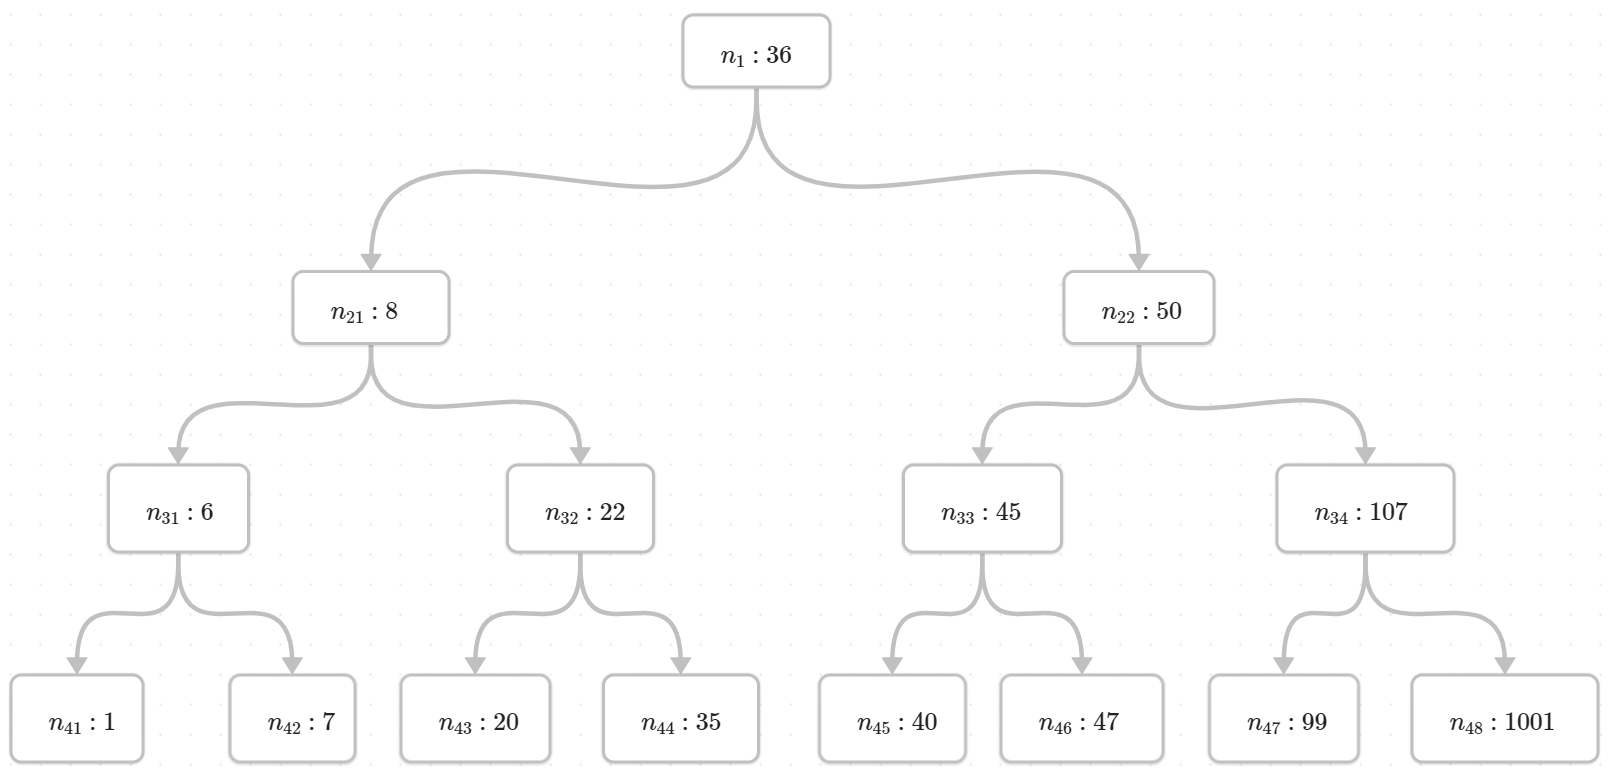
\includegraphics[width=0.9\textwidth]{tree.png}
    \caption{此二叉树的结构和内容}
  \end{center}
\end{figure}

同时,secret\_phase中还调用了函数fun7。可以写出函数func7等效的C代码。

\begin{lstlisting}[title = fun7对应的反汇编代码及注释, xleftmargin = 2em,xrightmargin = 2em, aboveskip = 1em, numbers = none, basicstyle=\footnotesize\ttfamily]
600 0000000000401204 <fun7>:
601   401204:   48 83 ec 08             sub    $0x8,%rsp                    ; %rsp -= 0x8;
602   401208:   48 85 ff                test   %rdi,%rdi                    ; if (%rdi == 0)
603   40120b:   74 2b                   je     401238 <fun7+0x34>           ;    goto #618;
604   40120d:   8b 17                   mov    (%rdi),%edx                  ; %edx = M[%rdi];
605   40120f:   39 f2                   cmp    %esi,%edx                    ; if (%edx <= %esi)
606   401211:   7e 0d                   jle    401220 <fun7+0x1c>           ;     goto #611;
607   401213:   48 8b 7f 08             mov    0x8(%rdi),%rdi               ; %rdi = M[%rdi + 0x8];
608   401217:   e8 e8 ff ff ff          callq  401204 <fun7>                ; fun7(%rdi, %rsi);
609   40121c:   01 c0                   add    %eax,%eax                    ; %eax += %eax;
610   40121e:   eb 1d                   jmp    40123d <fun7+0x39>           ; goto #619;
611   401220:   b8 00 00 00 00          mov    $0x0,%eax                    ; %eax = 0;
612   401225:   39 f2                   cmp    %esi,%edx                    ; if (%edx == %esi)
613   401227:   74 14                   je     40123d <fun7+0x39>           ;     goto #619;
614   401229:   48 8b 7f 10             mov    0x10(%rdi),%rdi              ; %rdi = M[%rdi + 0x10];
615   40122d:   e8 d2 ff ff ff          callq  401204 <fun7>                ; fun7(%rdi, %rsi);
616   401232:   8d 44 00 01             lea    0x1(%rax,%rax,1),%eax        ; %eax = 2 * %rax + 1;
617   401236:   eb 05                   jmp    40123d <fun7+0x39>           ; goto #619;
618   401238:   b8 ff ff ff ff          mov    $0xffffffff,%eax             ; %eax = -1;
619   40123d:   48 83 c4 08             add    $0x8,%rsp                    ; %rsp += 0x8;
620   401241:   c3                      retq                                ; return %rax;
\end{lstlisting}

\begin{lstlisting}[title = 与fun7等效的C代码, xleftmargin = 2em,xrightmargin = 2em, aboveskip = 1em, numbers = left, basicstyle=\small\ttfamily]
    typedef struct _node {
        int entry;
        node* left;
        node* right;
    } node;
    int fun7(node* a, int b) {
        int ret;
        if (a == NULL) {
                return -1;
            }
        if (a->entry <= b) {
            ret = 0;
            if (a->entry == b) {
                return 0;
            } else {
                ret = fun7(a->right, b);
                return 2 * ret + 1;
            }
        } else {
            ret = fun7(a->left, b);
            return 2 * ret;
        }   
    }
  \end{lstlisting}

可以发现,其实现了一个二叉树上的查找。在当前节点找到时返回0,在左孩子处找到时,返回$ret\times 2$,在右孩子处找到时,返回$ret \times 2 + 1$。

根据secret\_phase的汇编代码,我们可以得知,要想不引爆炸弹,需使fun7返回2。因此,需在$n_{32}$或$n_{43}$处找到。根据二叉树的内容,答案为“20”或“22”。
\normalsize
\subsection{实验步骤}
\large
\begin{enumerate}[1)]
  \item 解打包bomb.tar
        \begin{lstlisting}[language=bash]
    linux> tar -xvf bomb.tar
    \end{lstlisting}
  \item 阅读bomb.c源代码
  \item 对可执行程序bomb进行反汇编,生成bomb.s文件
        \begin{lstlisting}[language=bash]
    linux> objdump -d bomb > bomb.s
    \end{lstlisting}
  \item 阅读bomb.s文件中的汇编代码,对炸弹的每个阶段进行分析
  \item 使用gdb调试工具对bomb进行调试,进一步分析
        \begin{lstlisting}[language=bash]
    linux> gdb bomb
    \end{lstlisting}
\end{enumerate}
\normalsize
\section{实验过程与分析}
\large

实验的运行结果如下:
\begin{figure}[h]
  \centering
  % 在这里放你的图图
  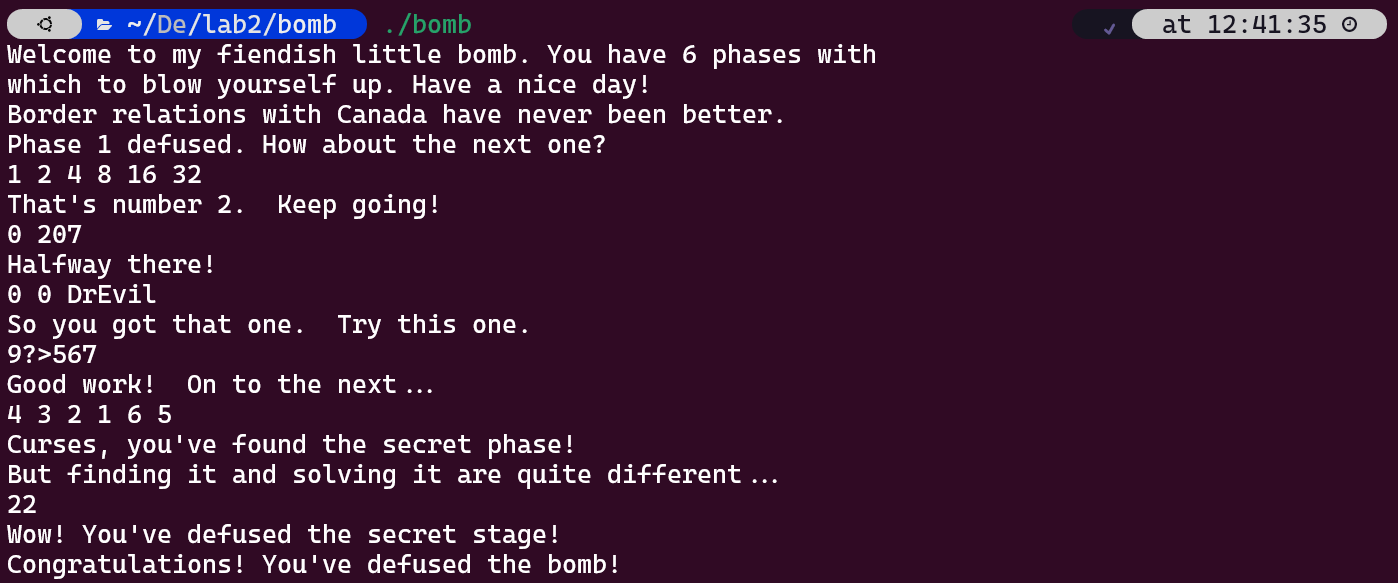
\includegraphics[width=15cm]{lab2.png}
  \caption{运行结果}
\end{figure}

\normalsize
\section{实验结果总结}
\large
在本次实验中,首先我学习到了反汇编工具objdump的使用,并用其生成了bomb的汇编文件。通过阅读汇编程序,我成功的破译了它的7个phase,在此过程中,我进一步加深了对汇编代码的理解,阅读汇编代码的能力也有所提高。

同时,我还学习到了gdb调试工具的基本应用,能用其解决一些简单的问题。
\normalsize
\section{附录(源代码)}
\large
bomb的反汇编代码及部分注释如下:

\begin{lstlisting}[title = bomb的反汇编代码及部分注释, xleftmargin = 2em,xrightmargin = 2em, aboveskip = 1em, numbers = left, basicstyle=\scriptsize\ttfamily, numberstyle=\scriptsize]

    bomb:     文件格式 elf64-x86-64


    Disassembly of section .init:
    
    0000000000400ac0 <_init>:
      400ac0:	48 83 ec 08          	sub    $0x8,%rsp
      400ac4:	e8 f3 01 00 00       	callq  400cbc <call_gmon_start>
      400ac9:	48 83 c4 08          	add    $0x8,%rsp
      400acd:	c3                   	retq   
    
    Disassembly of section .plt:
    
    0000000000400ad0 <.plt>:
      400ad0:	ff 35 1a 25 20 00    	pushq  0x20251a(%rip)        # 602ff0 <_GLOBAL_OFFSET_TABLE_+0x8>
      400ad6:	ff 25 1c 25 20 00    	jmpq   *0x20251c(%rip)        # 602ff8 <_GLOBAL_OFFSET_TABLE_+0x10>
      400adc:	0f 1f 40 00          	nopl   0x0(%rax)
    
    0000000000400ae0 <getenv@plt>:
      400ae0:	ff 25 1a 25 20 00    	jmpq   *0x20251a(%rip)        # 603000 <getenv@GLIBC_2.2.5>
      400ae6:	68 00 00 00 00       	pushq  $0x0
      400aeb:	e9 e0 ff ff ff       	jmpq   400ad0 <.plt>
    
    0000000000400af0 <__errno_location@plt>:
      400af0:	ff 25 12 25 20 00    	jmpq   *0x202512(%rip)        # 603008 <__errno_location@GLIBC_2.2.5>
      400af6:	68 01 00 00 00       	pushq  $0x1
      400afb:	e9 d0 ff ff ff       	jmpq   400ad0 <.plt>
    
    0000000000400b00 <strcpy@plt>:
      400b00:	ff 25 0a 25 20 00    	jmpq   *0x20250a(%rip)        # 603010 <strcpy@GLIBC_2.2.5>
      400b06:	68 02 00 00 00       	pushq  $0x2
      400b0b:	e9 c0 ff ff ff       	jmpq   400ad0 <.plt>
    
    0000000000400b10 <puts@plt>:
      400b10:	ff 25 02 25 20 00    	jmpq   *0x202502(%rip)        # 603018 <puts@GLIBC_2.2.5>
      400b16:	68 03 00 00 00       	pushq  $0x3
      400b1b:	e9 b0 ff ff ff       	jmpq   400ad0 <.plt>
    
    0000000000400b20 <write@plt>:
      400b20:	ff 25 fa 24 20 00    	jmpq   *0x2024fa(%rip)        # 603020 <write@GLIBC_2.2.5>
      400b26:	68 04 00 00 00       	pushq  $0x4
      400b2b:	e9 a0 ff ff ff       	jmpq   400ad0 <.plt>
    
    0000000000400b30 <__stack_chk_fail@plt>:
      400b30:	ff 25 f2 24 20 00    	jmpq   *0x2024f2(%rip)        # 603028 <__stack_chk_fail@GLIBC_2.4>
      400b36:	68 05 00 00 00       	pushq  $0x5
      400b3b:	e9 90 ff ff ff       	jmpq   400ad0 <.plt>
    
    0000000000400b40 <alarm@plt>:
      400b40:	ff 25 ea 24 20 00    	jmpq   *0x2024ea(%rip)        # 603030 <alarm@GLIBC_2.2.5>
      400b46:	68 06 00 00 00       	pushq  $0x6
      400b4b:	e9 80 ff ff ff       	jmpq   400ad0 <.plt>
    
    0000000000400b50 <close@plt>:
      400b50:	ff 25 e2 24 20 00    	jmpq   *0x2024e2(%rip)        # 603038 <close@GLIBC_2.2.5>
      400b56:	68 07 00 00 00       	pushq  $0x7
      400b5b:	e9 70 ff ff ff       	jmpq   400ad0 <.plt>
    
    0000000000400b60 <read@plt>:
      400b60:	ff 25 da 24 20 00    	jmpq   *0x2024da(%rip)        # 603040 <read@GLIBC_2.2.5>
      400b66:	68 08 00 00 00       	pushq  $0x8
      400b6b:	e9 60 ff ff ff       	jmpq   400ad0 <.plt>
    
    0000000000400b70 <__libc_start_main@plt>:
      400b70:	ff 25 d2 24 20 00    	jmpq   *0x2024d2(%rip)        # 603048 <__libc_start_main@GLIBC_2.2.5>
      400b76:	68 09 00 00 00       	pushq  $0x9
      400b7b:	e9 50 ff ff ff       	jmpq   400ad0 <.plt>
    
    0000000000400b80 <fgets@plt>:
      400b80:	ff 25 ca 24 20 00    	jmpq   *0x2024ca(%rip)        # 603050 <fgets@GLIBC_2.2.5>
      400b86:	68 0a 00 00 00       	pushq  $0xa
      400b8b:	e9 40 ff ff ff       	jmpq   400ad0 <.plt>
    
    0000000000400b90 <signal@plt>:
      400b90:	ff 25 c2 24 20 00    	jmpq   *0x2024c2(%rip)        # 603058 <signal@GLIBC_2.2.5>
      400b96:	68 0b 00 00 00       	pushq  $0xb
      400b9b:	e9 30 ff ff ff       	jmpq   400ad0 <.plt>
    
    0000000000400ba0 <gethostbyname@plt>:
      400ba0:	ff 25 ba 24 20 00    	jmpq   *0x2024ba(%rip)        # 603060 <gethostbyname@GLIBC_2.2.5>
      400ba6:	68 0c 00 00 00       	pushq  $0xc
      400bab:	e9 20 ff ff ff       	jmpq   400ad0 <.plt>
    
    0000000000400bb0 <__memmove_chk@plt>:
      400bb0:	ff 25 b2 24 20 00    	jmpq   *0x2024b2(%rip)        # 603068 <__memmove_chk@GLIBC_2.3.4>
      400bb6:	68 0d 00 00 00       	pushq  $0xd
      400bbb:	e9 10 ff ff ff       	jmpq   400ad0 <.plt>
    
    0000000000400bc0 <__memcpy_chk@plt>:
      400bc0:	ff 25 aa 24 20 00    	jmpq   *0x2024aa(%rip)        # 603070 <__memcpy_chk@GLIBC_2.3.4>
      400bc6:	68 0e 00 00 00       	pushq  $0xe
      400bcb:	e9 00 ff ff ff       	jmpq   400ad0 <.plt>
    
    0000000000400bd0 <strtol@plt>:
      400bd0:	ff 25 a2 24 20 00    	jmpq   *0x2024a2(%rip)        # 603078 <strtol@GLIBC_2.2.5>
      400bd6:	68 0f 00 00 00       	pushq  $0xf
      400bdb:	e9 f0 fe ff ff       	jmpq   400ad0 <.plt>
    
    0000000000400be0 <fflush@plt>:
      400be0:	ff 25 9a 24 20 00    	jmpq   *0x20249a(%rip)        # 603080 <fflush@GLIBC_2.2.5>
      400be6:	68 10 00 00 00       	pushq  $0x10
      400beb:	e9 e0 fe ff ff       	jmpq   400ad0 <.plt>
    
    0000000000400bf0 <__isoc99_sscanf@plt>:
      400bf0:	ff 25 92 24 20 00    	jmpq   *0x202492(%rip)        # 603088 <__isoc99_sscanf@GLIBC_2.7>
      400bf6:	68 11 00 00 00       	pushq  $0x11
      400bfb:	e9 d0 fe ff ff       	jmpq   400ad0 <.plt>
    
    0000000000400c00 <__printf_chk@plt>:
      400c00:	ff 25 8a 24 20 00    	jmpq   *0x20248a(%rip)        # 603090 <__printf_chk@GLIBC_2.3.4>
      400c06:	68 12 00 00 00       	pushq  $0x12
      400c0b:	e9 c0 fe ff ff       	jmpq   400ad0 <.plt>
    
    0000000000400c10 <fopen@plt>:
      400c10:	ff 25 82 24 20 00    	jmpq   *0x202482(%rip)        # 603098 <fopen@GLIBC_2.2.5>
      400c16:	68 13 00 00 00       	pushq  $0x13
      400c1b:	e9 b0 fe ff ff       	jmpq   400ad0 <.plt>
    
    0000000000400c20 <exit@plt>:
      400c20:	ff 25 7a 24 20 00    	jmpq   *0x20247a(%rip)        # 6030a0 <exit@GLIBC_2.2.5>
      400c26:	68 14 00 00 00       	pushq  $0x14
      400c2b:	e9 a0 fe ff ff       	jmpq   400ad0 <.plt>
    
    0000000000400c30 <connect@plt>:
      400c30:	ff 25 72 24 20 00    	jmpq   *0x202472(%rip)        # 6030a8 <connect@GLIBC_2.2.5>
      400c36:	68 15 00 00 00       	pushq  $0x15
      400c3b:	e9 90 fe ff ff       	jmpq   400ad0 <.plt>
    
    0000000000400c40 <__fprintf_chk@plt>:
      400c40:	ff 25 6a 24 20 00    	jmpq   *0x20246a(%rip)        # 6030b0 <__fprintf_chk@GLIBC_2.3.4>
      400c46:	68 16 00 00 00       	pushq  $0x16
      400c4b:	e9 80 fe ff ff       	jmpq   400ad0 <.plt>
    
    0000000000400c50 <sleep@plt>:
      400c50:	ff 25 62 24 20 00    	jmpq   *0x202462(%rip)        # 6030b8 <sleep@GLIBC_2.2.5>
      400c56:	68 17 00 00 00       	pushq  $0x17
      400c5b:	e9 70 fe ff ff       	jmpq   400ad0 <.plt>
    
    0000000000400c60 <__ctype_b_loc@plt>:
      400c60:	ff 25 5a 24 20 00    	jmpq   *0x20245a(%rip)        # 6030c0 <__ctype_b_loc@GLIBC_2.3>
      400c66:	68 18 00 00 00       	pushq  $0x18
      400c6b:	e9 60 fe ff ff       	jmpq   400ad0 <.plt>
    
    0000000000400c70 <__sprintf_chk@plt>:
      400c70:	ff 25 52 24 20 00    	jmpq   *0x202452(%rip)        # 6030c8 <__sprintf_chk@GLIBC_2.3.4>
      400c76:	68 19 00 00 00       	pushq  $0x19
      400c7b:	e9 50 fe ff ff       	jmpq   400ad0 <.plt>
    
    0000000000400c80 <socket@plt>:
      400c80:	ff 25 4a 24 20 00    	jmpq   *0x20244a(%rip)        # 6030d0 <socket@GLIBC_2.2.5>
      400c86:	68 1a 00 00 00       	pushq  $0x1a
      400c8b:	e9 40 fe ff ff       	jmpq   400ad0 <.plt>
    
    Disassembly of section .text:
    
    0000000000400c90 <_start>:
      400c90:	31 ed                	xor    %ebp,%ebp
      400c92:	49 89 d1             	mov    %rdx,%r9
      400c95:	5e                   	pop    %rsi
      400c96:	48 89 e2             	mov    %rsp,%rdx
      400c99:	48 83 e4 f0          	and    $0xfffffffffffffff0,%rsp
      400c9d:	50                   	push   %rax
      400c9e:	54                   	push   %rsp
      400c9f:	49 c7 c0 a0 22 40 00 	mov    $0x4022a0,%r8
      400ca6:	48 c7 c1 10 22 40 00 	mov    $0x402210,%rcx
      400cad:	48 c7 c7 a0 0d 40 00 	mov    $0x400da0,%rdi
      400cb4:	e8 b7 fe ff ff       	callq  400b70 <__libc_start_main@plt>
      400cb9:	f4                   	hlt    
      400cba:	90                   	nop
      400cbb:	90                   	nop
    
    0000000000400cbc <call_gmon_start>:
      400cbc:	48 83 ec 08          	sub    $0x8,%rsp
      400cc0:	48 8b 05 19 23 20 00 	mov    0x202319(%rip),%rax        # 602fe0 <__gmon_start__>
      400cc7:	48 85 c0             	test   %rax,%rax
      400cca:	74 02                	je     400cce <call_gmon_start+0x12>
      400ccc:	ff d0                	callq  *%rax
      400cce:	48 83 c4 08          	add    $0x8,%rsp
      400cd2:	c3                   	retq   
      400cd3:	90                   	nop
      400cd4:	90                   	nop
      400cd5:	90                   	nop
      400cd6:	90                   	nop
      400cd7:	90                   	nop
      400cd8:	90                   	nop
      400cd9:	90                   	nop
      400cda:	90                   	nop
      400cdb:	90                   	nop
      400cdc:	90                   	nop
      400cdd:	90                   	nop
      400cde:	90                   	nop
      400cdf:	90                   	nop
    
    0000000000400ce0 <deregister_tm_clones>:
      400ce0:	b8 47 37 60 00       	mov    $0x603747,%eax
      400ce5:	55                   	push   %rbp
      400ce6:	48 2d 40 37 60 00    	sub    $0x603740,%rax
      400cec:	48 83 f8 0e          	cmp    $0xe,%rax
      400cf0:	48 89 e5             	mov    %rsp,%rbp
      400cf3:	77 02                	ja     400cf7 <deregister_tm_clones+0x17>
      400cf5:	5d                   	pop    %rbp
      400cf6:	c3                   	retq   
      400cf7:	b8 00 00 00 00       	mov    $0x0,%eax
      400cfc:	48 85 c0             	test   %rax,%rax
      400cff:	74 f4                	je     400cf5 <deregister_tm_clones+0x15>
      400d01:	5d                   	pop    %rbp
      400d02:	bf 40 37 60 00       	mov    $0x603740,%edi
      400d07:	ff e0                	jmpq   *%rax
      400d09:	0f 1f 80 00 00 00 00 	nopl   0x0(%rax)
    
    0000000000400d10 <register_tm_clones>:
      400d10:	b8 40 37 60 00       	mov    $0x603740,%eax
      400d15:	55                   	push   %rbp
      400d16:	48 2d 40 37 60 00    	sub    $0x603740,%rax
      400d1c:	48 c1 f8 03          	sar    $0x3,%rax
      400d20:	48 89 e5             	mov    %rsp,%rbp
      400d23:	48 89 c2             	mov    %rax,%rdx
      400d26:	48 c1 ea 3f          	shr    $0x3f,%rdx
      400d2a:	48 01 d0             	add    %rdx,%rax
      400d2d:	48 d1 f8             	sar    %rax
      400d30:	75 02                	jne    400d34 <register_tm_clones+0x24>
      400d32:	5d                   	pop    %rbp
      400d33:	c3                   	retq   
      400d34:	ba 00 00 00 00       	mov    $0x0,%edx
      400d39:	48 85 d2             	test   %rdx,%rdx
      400d3c:	74 f4                	je     400d32 <register_tm_clones+0x22>
      400d3e:	5d                   	pop    %rbp
      400d3f:	48 89 c6             	mov    %rax,%rsi
      400d42:	bf 40 37 60 00       	mov    $0x603740,%edi
      400d47:	ff e2                	jmpq   *%rdx
      400d49:	0f 1f 80 00 00 00 00 	nopl   0x0(%rax)
    
    0000000000400d50 <__do_global_dtors_aux>:
      400d50:	80 3d 01 2a 20 00 00 	cmpb   $0x0,0x202a01(%rip)        # 603758 <completed.6976>
      400d57:	75 11                	jne    400d6a <__do_global_dtors_aux+0x1a>
      400d59:	55                   	push   %rbp
      400d5a:	48 89 e5             	mov    %rsp,%rbp
      400d5d:	e8 7e ff ff ff       	callq  400ce0 <deregister_tm_clones>
      400d62:	5d                   	pop    %rbp
      400d63:	c6 05 ee 29 20 00 01 	movb   $0x1,0x2029ee(%rip)        # 603758 <completed.6976>
      400d6a:	f3 c3                	repz retq 
      400d6c:	0f 1f 40 00          	nopl   0x0(%rax)
    
    0000000000400d70 <frame_dummy>:
      400d70:	48 83 3d 90 20 20 00 	cmpq   $0x0,0x202090(%rip)        # 602e08 <__JCR_END__>
      400d77:	00 
      400d78:	74 1e                	je     400d98 <frame_dummy+0x28>
      400d7a:	b8 00 00 00 00       	mov    $0x0,%eax
      400d7f:	48 85 c0             	test   %rax,%rax
      400d82:	74 14                	je     400d98 <frame_dummy+0x28>
      400d84:	55                   	push   %rbp
      400d85:	bf 08 2e 60 00       	mov    $0x602e08,%edi
      400d8a:	48 89 e5             	mov    %rsp,%rbp
      400d8d:	ff d0                	callq  *%rax
      400d8f:	5d                   	pop    %rbp
      400d90:	e9 7b ff ff ff       	jmpq   400d10 <register_tm_clones>
      400d95:	0f 1f 00             	nopl   (%rax)
      400d98:	e9 73 ff ff ff       	jmpq   400d10 <register_tm_clones>
      400d9d:	90                   	nop
      400d9e:	90                   	nop
      400d9f:	90                   	nop
    
    0000000000400da0 <main>:
      400da0:	53                   	push   %rbx
      400da1:	83 ff 01             	cmp    $0x1,%edi
      400da4:	75 10                	jne    400db6 <main+0x16>
      400da6:	48 8b 05 9b 29 20 00 	mov    0x20299b(%rip),%rax        # 603748 <stdin@@GLIBC_2.2.5>
      400dad:	48 89 05 b4 29 20 00 	mov    %rax,0x2029b4(%rip)        # 603768 <infile>
      400db4:	eb 63                	jmp    400e19 <main+0x79>
      400db6:	48 89 f3             	mov    %rsi,%rbx
      400db9:	83 ff 02             	cmp    $0x2,%edi
      400dbc:	75 3a                	jne    400df8 <main+0x58>
      400dbe:	48 8b 7e 08          	mov    0x8(%rsi),%rdi
      400dc2:	be b4 22 40 00       	mov    $0x4022b4,%esi
      400dc7:	e8 44 fe ff ff       	callq  400c10 <fopen@plt>
      400dcc:	48 89 05 95 29 20 00 	mov    %rax,0x202995(%rip)        # 603768 <infile>
      400dd3:	48 85 c0             	test   %rax,%rax
      400dd6:	75 41                	jne    400e19 <main+0x79>
      400dd8:	48 8b 4b 08          	mov    0x8(%rbx),%rcx
      400ddc:	48 8b 13             	mov    (%rbx),%rdx
      400ddf:	be b6 22 40 00       	mov    $0x4022b6,%esi
      400de4:	bf 01 00 00 00       	mov    $0x1,%edi
      400de9:	e8 12 fe ff ff       	callq  400c00 <__printf_chk@plt>
      400dee:	bf 08 00 00 00       	mov    $0x8,%edi
      400df3:	e8 28 fe ff ff       	callq  400c20 <exit@plt>
      400df8:	48 8b 16             	mov    (%rsi),%rdx
      400dfb:	be d3 22 40 00       	mov    $0x4022d3,%esi
      400e00:	bf 01 00 00 00       	mov    $0x1,%edi
      400e05:	b8 00 00 00 00       	mov    $0x0,%eax
      400e0a:	e8 f1 fd ff ff       	callq  400c00 <__printf_chk@plt>
      400e0f:	bf 08 00 00 00       	mov    $0x8,%edi
      400e14:	e8 07 fe ff ff       	callq  400c20 <exit@plt>
      400e19:	e8 84 05 00 00       	callq  4013a2 <initialize_bomb>
      400e1e:	bf 38 23 40 00       	mov    $0x402338,%edi
      400e23:	e8 e8 fc ff ff       	callq  400b10 <puts@plt>
      400e28:	bf 78 23 40 00       	mov    $0x402378,%edi
      400e2d:	e8 de fc ff ff       	callq  400b10 <puts@plt>
      400e32:	e8 67 06 00 00       	callq  40149e <read_line>
      400e37:	48 89 c7             	mov    %rax,%rdi
      400e3a:	e8 a1 00 00 00       	callq  400ee0 <phase_1>
      400e3f:	e8 80 07 00 00       	callq  4015c4 <phase_defused>
      400e44:	bf a8 23 40 00       	mov    $0x4023a8,%edi
      400e49:	e8 c2 fc ff ff       	callq  400b10 <puts@plt>
      400e4e:	e8 4b 06 00 00       	callq  40149e <read_line>
      400e53:	48 89 c7             	mov    %rax,%rdi
      400e56:	e8 a1 00 00 00       	callq  400efc <phase_2>
      400e5b:	e8 64 07 00 00       	callq  4015c4 <phase_defused>
      400e60:	bf ed 22 40 00       	mov    $0x4022ed,%edi
      400e65:	e8 a6 fc ff ff       	callq  400b10 <puts@plt>
      400e6a:	e8 2f 06 00 00       	callq  40149e <read_line>
      400e6f:	48 89 c7             	mov    %rax,%rdi
      400e72:	e8 cc 00 00 00       	callq  400f43 <phase_3>
      400e77:	e8 48 07 00 00       	callq  4015c4 <phase_defused>
      400e7c:	bf 0b 23 40 00       	mov    $0x40230b,%edi
      400e81:	e8 8a fc ff ff       	callq  400b10 <puts@plt>
      400e86:	e8 13 06 00 00       	callq  40149e <read_line>
      400e8b:	48 89 c7             	mov    %rax,%rdi
      400e8e:	e8 79 01 00 00       	callq  40100c <phase_4>
      400e93:	e8 2c 07 00 00       	callq  4015c4 <phase_defused>
      400e98:	bf d8 23 40 00       	mov    $0x4023d8,%edi
      400e9d:	e8 6e fc ff ff       	callq  400b10 <puts@plt>
      400ea2:	e8 f7 05 00 00       	callq  40149e <read_line>
      400ea7:	48 89 c7             	mov    %rax,%rdi
      400eaa:	e8 b3 01 00 00       	callq  401062 <phase_5>
      400eaf:	e8 10 07 00 00       	callq  4015c4 <phase_defused>
      400eb4:	bf 1a 23 40 00       	mov    $0x40231a,%edi
      400eb9:	e8 52 fc ff ff       	callq  400b10 <puts@plt>
      400ebe:	e8 db 05 00 00       	callq  40149e <read_line>
      400ec3:	48 89 c7             	mov    %rax,%rdi
      400ec6:	e8 29 02 00 00       	callq  4010f4 <phase_6>
      400ecb:	e8 f4 06 00 00       	callq  4015c4 <phase_defused>
      400ed0:	b8 00 00 00 00       	mov    $0x0,%eax
      400ed5:	5b                   	pop    %rbx
      400ed6:	c3                   	retq   
      400ed7:	90                   	nop
      400ed8:	90                   	nop
      400ed9:	90                   	nop
      400eda:	90                   	nop
      400edb:	90                   	nop
      400edc:	90                   	nop
      400edd:	90                   	nop
      400ede:	90                   	nop
      400edf:	90                   	nop
    
    0000000000400ee0 <phase_1>:
      400ee0:	48 83 ec 08          	sub    $0x8,%rsp					; %rsp -= 0x8;
      400ee4:	be 00 24 40 00       	mov    $0x402400,%esi				; %esi = 0x402400;
      400ee9:	e8 4a 04 00 00       	callq  401338 <strings_not_equal>	; strings_not_equal(...);
      400eee:	85 c0                	test   %eax,%eax					; if (%eax != 0)
      400ef0:	74 05                	je     400ef7 <phase_1+0x17>		;     goto #351;
      400ef2:	e8 43 05 00 00       	callq  40143a <explode_bomb>		; explode_bomb(...)
      400ef7:	48 83 c4 08          	add    $0x8,%rsp					; %rsp += 8;
      400efb:	c3                   	retq								; return;
    
    0000000000400efc <phase_2>:
      400efc:	55                   	push   %rbp
      400efd:	53                   	push   %rbx
      400efe:	48 83 ec 28          	sub    $0x28,%rsp					; %rsp -= 0x28;
      400f02:	48 89 e6             	mov    %rsp,%rsi					; %rsi = %rsp;
      400f05:	e8 52 05 00 00       	callq  40145c <read_six_numbers>	; read_six_numbers(...);
      400f0a:	83 3c 24 01          	cmpl   $0x1,(%rsp)					; if (M[%rsp] == 1)
      400f0e:	74 20                	je     400f30 <phase_2+0x34>		;	  goto #375;
      400f10:	e8 25 05 00 00       	callq  40143a <explode_bomb>		; explode_bomb(...);
      400f15:	eb 19                	jmp    400f30 <phase_2+0x34>		; goto #375;
      400f17:	8b 43 fc             	mov    -0x4(%rbx),%eax				; %eax = M[%rbx - 4];
      400f1a:	01 c0                	add    %eax,%eax					; %eax += %eax;
      400f1c:	39 03                	cmp    %eax,(%rbx)					; if (%eax == M[%rbx])
      400f1e:	74 05                	je     400f25 <phase_2+0x29>		;	  goto #371;
      400f20:	e8 15 05 00 00       	callq  40143a <explode_bomb>		; explode_bomb(...);
      400f25:	48 83 c3 04          	add    $0x4,%rbx					; %rbx += 4;
      400f29:	48 39 eb             	cmp    %rbp,%rbx					; if (%rbp != %rbx)
      400f2c:	75 e9                	jne    400f17 <phase_2+0x1b>		;	  goto #366;
      400f2e:	eb 0c                	jmp    400f3c <phase_2+0x40>		; goto #378;
      400f30:	48 8d 5c 24 04       	lea    0x4(%rsp),%rbx				; %rbx = %rsp + 0x4;
      400f35:	48 8d 6c 24 18       	lea    0x18(%rsp),%rbp				; %rbp = %rsp + 0x18;
      400f3a:	eb db                	jmp    400f17 <phase_2+0x1b>		; goto #366;
      400f3c:	48 83 c4 28          	add    $0x28,%rsp					; %rsp += 0x28;
      400f40:	5b                   	pop    %rbx
      400f41:	5d                   	pop    %rbp
      400f42:	c3                   	retq   
    
    0000000000400f43 <phase_3>:
      400f43:	48 83 ec 18          	sub    $0x18,%rsp					; %rsp -= 0x18;
      400f47:	48 8d 4c 24 0c       	lea    0xc(%rsp),%rcx				; %rcx = %rsp + 0xc;
      400f4c:	48 8d 54 24 08       	lea    0x8(%rsp),%rdx				; %rdx = %rsp + 0x8;
      400f51:	be cf 25 40 00       	mov    $0x4025cf,%esi				; %esi = 0x4025cf;
      400f56:	b8 00 00 00 00       	mov    $0x0,%eax					; %eax = 0;
      400f5b:	e8 90 fc ff ff       	callq  400bf0 <__isoc99_sscanf@plt>	; sscanf(...)
      400f60:	83 f8 01             	cmp    $0x1,%eax					; if (%eax > 1)
      400f63:	7f 05                	jg     400f6a <phase_3+0x27>		;	  goto #393;
      400f65:	e8 d0 04 00 00       	callq  40143a <explode_bomb>		; explode_bomb;
      400f6a:	83 7c 24 08 07       	cmpl   $0x7,0x8(%rsp)				; if (M[%rsp + 0x8] > 7)
      400f6f:	77 3c                	ja     400fad <phase_3+0x6a>		;	  goto #411;
      400f71:	8b 44 24 08          	mov    0x8(%rsp),%eax				; %eax = M[%rsp + 0x8];
      400f75:	ff 24 c5 70 24 40 00 	jmpq   *0x402470(,%rax,8)			; goto 8 * %rax + 0x402470;
      400f7c:	b8 cf 00 00 00       	mov    $0xcf,%eax				; 0:  %eax = 0xcf;
      400f81:	eb 3b                	jmp    400fbe <phase_3+0x7b>		; goto #415;
      400f83:	b8 c3 02 00 00       	mov    $0x2c3,%eax				; 2:  %eax = 0x2c3;	
      400f88:	eb 34                	jmp    400fbe <phase_3+0x7b>		; goto #415;
      400f8a:	b8 00 01 00 00       	mov    $0x100,%eax				; 3:  %eax = 0x100;
      400f8f:	eb 2d                	jmp    400fbe <phase_3+0x7b>		; goto #415;
      400f91:	b8 85 01 00 00       	mov    $0x185,%eax				; 4:  %eax = 0x185;
      400f96:	eb 26                	jmp    400fbe <phase_3+0x7b>		; goto #415;
      400f98:	b8 ce 00 00 00       	mov    $0xce,%eax				; 5:  %eax = 0xce;
      400f9d:	eb 1f                	jmp    400fbe <phase_3+0x7b>		; goto #415;
      400f9f:	b8 aa 02 00 00       	mov    $0x2aa,%eax				; 6:  %eax = 0x2aa;
      400fa4:	eb 18                	jmp    400fbe <phase_3+0x7b>		; goto #415;
      400fa6:	b8 47 01 00 00       	mov    $0x147,%eax				; 7:  %eax = 0x147;
      400fab:	eb 11                	jmp    400fbe <phase_3+0x7b>		; goto #415;
      400fad:	e8 88 04 00 00       	callq  40143a <explode_bomb>		; explode_bomb(...);
      400fb2:	b8 00 00 00 00       	mov    $0x0,%eax					; %eax = 0;
      400fb7:	eb 05                	jmp    400fbe <phase_3+0x7b>		; goto #415;
      400fb9:	b8 37 01 00 00       	mov    $0x137,%eax				; 1:  %eax = 0x137;
      400fbe:	3b 44 24 0c          	cmp    0xc(%rsp),%eax				; if (%eax == M[%rsp + 0xc])
      400fc2:	74 05                	je     400fc9 <phase_3+0x86>		;	  goto #418;
      400fc4:	e8 71 04 00 00       	callq  40143a <explode_bomb>		; explode_bomb(...);
      400fc9:	48 83 c4 18          	add    $0x18,%rsp					; %rsp += 0x18;
      400fcd:	c3                   	retq								; return;
    
    0000000000400fce <func4>:
      400fce:	48 83 ec 08          	sub    $0x8,%rsp					; %rsp -= 0x8;
      400fd2:	89 d0                	mov    %edx,%eax					; %eax = %rdx;
      400fd4:	29 f0                	sub    %esi,%eax					; %eax -= %esi;
      400fd6:	89 c1                	mov    %eax,%ecx					; %ecx = %eax;
      400fd8:	c1 e9 1f             	shr    $0x1f,%ecx					; %ecx >>=(H) 0x1f;
      400fdb:	01 c8                	add    %ecx,%eax					; %eax += %ecx;
      400fdd:	d1 f8                	sar    %eax							; %eax >>= 1;
      400fdf:	8d 0c 30             	lea    (%rax,%rsi,1),%ecx			; %ecx = %rax + %rsi;
      400fe2:	39 f9                	cmp    %edi,%ecx					; if (%ecx <= %edi)
      400fe4:	7e 0c                	jle    400ff2 <func4+0x24>			;	  goto #436;
      400fe6:	8d 51 ff             	lea    -0x1(%rcx),%edx				; %edx = %rcx - 1;
      400fe9:	e8 e0 ff ff ff       	callq  400fce <func4>				; func4(%rdi, %rsi, %rdx);
      400fee:	01 c0                	add    %eax,%eax					; %eax += %eax;
      400ff0:	eb 15                	jmp    401007 <func4+0x39>			; goto #442;
      400ff2:	b8 00 00 00 00       	mov    $0x0,%eax					; %eax = 0;
      400ff7:	39 f9                	cmp    %edi,%ecx					; if (%ecx >= %edi)
      400ff9:	7d 0c                	jge    401007 <func4+0x39>			;	  goto #442;
      400ffb:	8d 71 01             	lea    0x1(%rcx),%esi				; %esi = %rcx + 1;
      400ffe:	e8 cb ff ff ff       	callq  400fce <func4>				; func4(%rdi, %rsi, %rdx);
      401003:	8d 44 00 01          	lea    0x1(%rax,%rax,1),%eax		; %eax = 2 * %rax + 1;
      401007:	48 83 c4 08          	add    $0x8,%rsp					; %rsp += 8;
      40100b:	c3                   	retq								; return %eax;
    
    000000000040100c <phase_4>:
      40100c:	48 83 ec 18          	sub    $0x18,%rsp					; %rsp -= 0x18;
      401010:	48 8d 4c 24 0c       	lea    0xc(%rsp),%rcx				; %rcx = %rsp + 0xc;
      401015:	48 8d 54 24 08       	lea    0x8(%rsp),%rdx				; %rdx = %rsp + 0x8;
      40101a:	be cf 25 40 00       	mov    $0x4025cf,%esi				; %esi = 0x4025cf;
      40101f:	b8 00 00 00 00       	mov    $0x0,%eax					; %eax = 0;
      401024:	e8 c7 fb ff ff       	callq  400bf0 <__isoc99_sscanf@plt>	; sscanf(...)
      401029:	83 f8 02             	cmp    $0x2,%eax					; if (%eax != 2)
      40102c:	75 07                	jne    401035 <phase_4+0x29>		;	  goto #456;
      40102e:	83 7c 24 08 0e       	cmpl   $0xe,0x8(%rsp)				; if (M[%rsp + 0x8] <= 0xe)
      401033:	76 05                	jbe    40103a <phase_4+0x2e>		;	  goto #457;
      401035:	e8 00 04 00 00       	callq  40143a <explode_bomb>		; explode_bomb(...);
      40103a:	ba 0e 00 00 00       	mov    $0xe,%edx					; %edx = 0xe;
      40103f:	be 00 00 00 00       	mov    $0x0,%esi					; %rsi = 0;
      401044:	8b 7c 24 08          	mov    0x8(%rsp),%edi				; %edi = M[%rsp + 0x8];
      401048:	e8 81 ff ff ff       	callq  400fce <func4>				; func4(%edi, %esi, %edx);
      40104d:	85 c0                	test   %eax,%eax					; if (%eax != 0)
      40104f:	75 07                	jne    401058 <phase_4+0x4c>		;	  goto #465;
      401051:	83 7c 24 0c 00       	cmpl   $0x0,0xc(%rsp)				; if (M[%rsp + 0xc] == 0)
      401056:	74 05                	je     40105d <phase_4+0x51>		;	  goto #466;
      401058:	e8 dd 03 00 00       	callq  40143a <explode_bomb>		; explode_bomb(...);
      40105d:	48 83 c4 18          	add    $0x18,%rsp					; %rsp += 0x18;
      401061:	c3                   	retq								; return;
    
    0000000000401062 <phase_5>:
      401062:	53                   	push   %rbx							
      401063:	48 83 ec 20          	sub    $0x20,%rsp					; %rsp -= 0x20;
      401067:	48 89 fb             	mov    %rdi,%rbx					; %rbx = %rdi;
      40106a:	64 48 8b 04 25 28 00 	mov    %fs:0x28,%rax				; %rax = 0x28;
      401071:	00 00 
      401073:	48 89 44 24 18       	mov    %rax,0x18(%rsp)				; M[%rsp + 0x18] = %rax;
      401078:	31 c0                	xor    %eax,%eax					; %eax ^= %eax;
      40107a:	e8 9c 02 00 00       	callq  40131b <string_length>		; string_length(%rdi);
      40107f:	83 f8 06             	cmp    $0x6,%eax					; if (%eax == 6)
      401082:	74 4e                	je     4010d2 <phase_5+0x70>		;	  goto #500;
      401084:	e8 b1 03 00 00       	callq  40143a <explode_bomb>		; explode_bomb(...);
      401089:	eb 47                	jmp    4010d2 <phase_5+0x70>		; goto #500;
      40108b:	0f b6 0c 03          	movzbl (%rbx,%rax,1),%ecx			; %ecx = %rbx + %rax;
      40108f:	88 0c 24             	mov    %cl,(%rsp)					; M[%rsp] = %cl;
      401092:	48 8b 14 24          	mov    (%rsp),%rdx					; %rdx = M[%rsp];
      401096:	83 e2 0f             	and    $0xf,%edx					; %edx &= 0xf;
      401099:	0f b6 92 b0 24 40 00 	movzbl 0x4024b0(%rdx),%edx			; %edx = M[%rdx + 0x4024b0];
      4010a0:	88 54 04 10          	mov    %dl,0x10(%rsp,%rax,1)		; M[%rsp + %rax + 0x10] = %dl; 
      4010a4:	48 83 c0 01          	add    $0x1,%rax					; %rax++;
      4010a8:	48 83 f8 06          	cmp    $0x6,%rax					; if (%rax != 0x6)
      4010ac:	75 dd                	jne    40108b <phase_5+0x29>		;	  goto #482;
      4010ae:	c6 44 24 16 00       	movb   $0x0,0x16(%rsp)				; M[%rsp + 0x16] = 0;
      4010b3:	be 5e 24 40 00       	mov    $0x40245e,%esi				; %esi = 0x40245e;
      4010b8:	48 8d 7c 24 10       	lea    0x10(%rsp),%rdi				; %rdi = %rsp + 0x10;
      4010bd:	e8 76 02 00 00       	callq  401338 <strings_not_equal>	; strings_not_equal(%rdi, %rsi);
      4010c2:	85 c0                	test   %eax,%eax					; if (%eax == 0)
      4010c4:	74 13                	je     4010d9 <phase_5+0x77>		;	  goto #502;
      4010c6:	e8 6f 03 00 00       	callq  40143a <explode_bomb>		; explode_bomb(...);
      4010cb:	0f 1f 44 00 00       	nopl   0x0(%rax,%rax,1)				; ???
      4010d0:	eb 07                	jmp    4010d9 <phase_5+0x77>		; goto #502;
      4010d2:	b8 00 00 00 00       	mov    $0x0,%eax					; %eax = 0;
      4010d7:	eb b2                	jmp    40108b <phase_5+0x29>		; goto #482;
      4010d9:	48 8b 44 24 18       	mov    0x18(%rsp),%rax				; %rax = M[%rsp + 0x18];
      4010de:	64 48 33 04 25 28 00 	xor    %fs:0x28,%rax				; %rax ^= 0x28;
      4010e5:	00 00 
      4010e7:	74 05                	je     4010ee <phase_5+0x8c>		; goto #507;
      4010e9:	e8 42 fa ff ff       	callq  400b30 <__stack_chk_fail@plt>; 
      4010ee:	48 83 c4 20          	add    $0x20,%rsp					; %rsp += 0x20;
      4010f2:	5b                   	pop    %rbx
      4010f3:	c3                   	retq   
    
    00000000004010f4 <phase_6>:
      4010f4:	41 56                	push   %r14
      4010f6:	41 55                	push   %r13
      4010f8:	41 54                	push   %r12
      4010fa:	55                   	push   %rbp
      4010fb:	53                   	push   %rbx
      4010fc:	48 83 ec 50          	sub    $0x50,%rsp					; %rsp -= 0x50;
      401100:	49 89 e5             	mov    %rsp,%r13					; %r13 = %rsp; 
      401103:	48 89 e6             	mov    %rsp,%rsi					; %rsi = %rsp;
      401106:	e8 51 03 00 00       	callq  40145c <read_six_numbers>	; read_six_numbers(...);
      40110b:	49 89 e6             	mov    %rsp,%r14					; %r14 = %rsp;
      40110e:	41 bc 00 00 00 00    	mov    $0x0,%r12d					; %r12d = 0;
      401114:	4c 89 ed             	mov    %r13,%rbp					; %rbp = %r13;
      401117:	41 8b 45 00          	mov    0x0(%r13),%eax				; %eax = M[%r13];
      40111b:	83 e8 01             	sub    $0x1,%eax					; %eax--;
      40111e:	83 f8 05             	cmp    $0x5,%eax					; if (%eax <= 5)
      401121:	76 05                	jbe    401128 <phase_6+0x34>		;	  goto #529;
      401123:	e8 12 03 00 00       	callq  40143a <explode_bomb>		; explode_bomb(...);
      401128:	41 83 c4 01          	add    $0x1,%r12d					; %r12d++;
      40112c:	41 83 fc 06          	cmp    $0x6,%r12d					; if (%r12d == 6)
      401130:	74 21                	je     401153 <phase_6+0x5f>		;	  goto #543;
      401132:	44 89 e3             	mov    %r12d,%ebx					; %ebx = %r12d;
      401135:	48 63 c3             	movslq %ebx,%rax					; %rax = %ebx;
      401138:	8b 04 84             	mov    (%rsp,%rax,4),%eax			; %eax = M[%rsp + %eax * 4];
      40113b:	39 45 00             	cmp    %eax,0x0(%rbp)				; if (M[%rbp] != %eax)
      40113e:	75 05                	jne    401145 <phase_6+0x51>		;	  goto #538;
      401140:	e8 f5 02 00 00       	callq  40143a <explode_bomb>		; explode_bomb(...);
      401145:	83 c3 01             	add    $0x1,%ebx					; %ebx++;
      401148:	83 fb 05             	cmp    $0x5,%ebx					; if (%ebx <= 5)
      40114b:	7e e8                	jle    401135 <phase_6+0x41>		;	  goto #533;
      40114d:	49 83 c5 04          	add    $0x4,%r13					; %r13 += 4;
      401151:	eb c1                	jmp    401114 <phase_6+0x20>		; goto #523;
      401153:	48 8d 74 24 18       	lea    0x18(%rsp),%rsi				; %rsi = %rsp + 0x18;
      401158:	4c 89 f0             	mov    %r14,%rax					; %rax = %r14;
      40115b:	b9 07 00 00 00       	mov    $0x7,%ecx					; %ecx = 0x7;
      401160:	89 ca                	mov    %ecx,%edx					; %edx = %ecx;
      401162:	2b 10                	sub    (%rax),%edx					; %edx -= M[%rax];
      401164:	89 10                	mov    %edx,(%rax)					; M[%rax] = %edx;
      401166:	48 83 c0 04          	add    $0x4,%rax					; %rax += 4;
      40116a:	48 39 f0             	cmp    %rsi,%rax					; if (%rax != %rsi)
      40116d:	75 f1                	jne    401160 <phase_6+0x6c>		;	  goto #546;
      40116f:	be 00 00 00 00       	mov    $0x0,%esi					; %esi = 0;
      401174:	eb 21                	jmp    401197 <phase_6+0xa3>		; goto #564;
      401176:	48 8b 52 08          	mov    0x8(%rdx),%rdx				; %rdx = M[%rdx + 8];
      40117a:	83 c0 01             	add    $0x1,%eax					; %eax++;
      40117d:	39 c8                	cmp    %ecx,%eax					; if (%eax != %ecx)
      40117f:	75 f5                	jne    401176 <phase_6+0x82>		;	  goto #554;
      401181:	eb 05                	jmp    401188 <phase_6+0x94>		; goto #560;
      401183:	ba d0 32 60 00       	mov    $0x6032d0,%edx				; %edx = 0x6032d0;
      401188:	48 89 54 74 20       	mov    %rdx,0x20(%rsp,%rsi,2)		; M[%rsp + %rsi * 2 + 0x20] = %rdx;
      40118d:	48 83 c6 04          	add    $0x4,%rsi					; %rsi += 4;
      401191:	48 83 fe 18          	cmp    $0x18,%rsi					; if (%rsi == 0x18)
      401195:	74 14                	je     4011ab <phase_6+0xb7>		;	  goto #570;
      401197:	8b 0c 34             	mov    (%rsp,%rsi,1),%ecx			; %ecx = M[%rsp + %rsi];
      40119a:	83 f9 01             	cmp    $0x1,%ecx					; if (%ecx <= 1)
      40119d:	7e e4                	jle    401183 <phase_6+0x8f>		;	  goto #559;
      40119f:	b8 01 00 00 00       	mov    $0x1,%eax					; %eax = 1;
      4011a4:	ba d0 32 60 00       	mov    $0x6032d0,%edx				; %edx = 0x6032d0;
      4011a9:	eb cb                	jmp    401176 <phase_6+0x82>		; goto #554;
      4011ab:	48 8b 5c 24 20       	mov    0x20(%rsp),%rbx				; %rbx = M[%rsp + 0x20];
      4011b0:	48 8d 44 24 28       	lea    0x28(%rsp),%rax				; %rax = %rsp + 0x28;
      4011b5:	48 8d 74 24 50       	lea    0x50(%rsp),%rsi				; %rsi = %rsp + 0x50;
      4011ba:	48 89 d9             	mov    %rbx,%rcx					; %rcx = %rbx;
      4011bd:	48 8b 10             	mov    (%rax),%rdx					; %rdx = M[%rax];
      4011c0:	48 89 51 08          	mov    %rdx,0x8(%rcx)				; M[%rcx + 0x8] = %rdx;
      4011c4:	48 83 c0 08          	add    $0x8,%rax					; %rax += 8;
      4011c8:	48 39 f0             	cmp    %rsi,%rax					; if (%rax == %rsi)
      4011cb:	74 05                	je     4011d2 <phase_6+0xde>		;	  goto #581;
      4011cd:	48 89 d1             	mov    %rdx,%rcx					; %rcx = %rdx;
      4011d0:	eb eb                	jmp    4011bd <phase_6+0xc9>		; goto #574;
      4011d2:	48 c7 42 08 00 00 00 	movq   $0x0,0x8(%rdx)				; M[%rdx + 8] = 0;
      4011d9:	00 
      4011da:	bd 05 00 00 00       	mov    $0x5,%ebp					; %ebp = 5;
      4011df:	48 8b 43 08          	mov    0x8(%rbx),%rax				; %rax = M[%rbx + 8];
      4011e3:	8b 00                	mov    (%rax),%eax					; %eax = M[%rax];
      4011e5:	39 03                	cmp    %eax,(%rbx)					; if (M[%rbx] >= %eax)
      4011e7:	7d 05                	jge    4011ee <phase_6+0xfa>		;	  goto #589;
      4011e9:	e8 4c 02 00 00       	callq  40143a <explode_bomb>		; explode_bomb(...);
      4011ee:	48 8b 5b 08          	mov    0x8(%rbx),%rbx				; %rbx = M[%rbx + 8];
      4011f2:	83 ed 01             	sub    $0x1,%ebp					; %ebp--;
      4011f5:	75 e8                	jne    4011df <phase_6+0xeb>		; goto #584;
      4011f7:	48 83 c4 50          	add    $0x50,%rsp					; %rsp += 0x50;
      4011fb:	5b                   	pop    %rbx
      4011fc:	5d                   	pop    %rbp
      4011fd:	41 5c                	pop    %r12
      4011ff:	41 5d                	pop    %r13
      401201:	41 5e                	pop    %r14
      401203:	c3                   	retq   
    
    0000000000401204 <fun7>:
      401204:	48 83 ec 08          	sub    $0x8,%rsp					; %rsp -= 0x8;
      401208:	48 85 ff             	test   %rdi,%rdi					; if (%rdi == 0)
      40120b:	74 2b                	je     401238 <fun7+0x34>			;    goto #618;
      40120d:	8b 17                	mov    (%rdi),%edx					; %edx = M[%rdi];
      40120f:	39 f2                	cmp    %esi,%edx					; if (%edx <= %esi)
      401211:	7e 0d                	jle    401220 <fun7+0x1c>			;	  goto #611;
      401213:	48 8b 7f 08          	mov    0x8(%rdi),%rdi				; %rdi = M[%rdi + 0x8];
      401217:	e8 e8 ff ff ff       	callq  401204 <fun7>				; fun7(%rdi, %rsi);
      40121c:	01 c0                	add    %eax,%eax					; %eax += %eax;
      40121e:	eb 1d                	jmp    40123d <fun7+0x39>			; goto #619;
      401220:	b8 00 00 00 00       	mov    $0x0,%eax					; %eax = 0;
      401225:	39 f2                	cmp    %esi,%edx					; if (%edx == %esi)
      401227:	74 14                	je     40123d <fun7+0x39>			;     goto #619;
      401229:	48 8b 7f 10          	mov    0x10(%rdi),%rdi				; %rdi = M[%rdi + 0x10];
      40122d:	e8 d2 ff ff ff       	callq  401204 <fun7>				; fun7(%rdi, %rsi);
      401232:	8d 44 00 01          	lea    0x1(%rax,%rax,1),%eax		; %eax = 2 * %rax + 1;
      401236:	eb 05                	jmp    40123d <fun7+0x39>			; goto #619;
      401238:	b8 ff ff ff ff       	mov    $0xffffffff,%eax				; %eax = -1;
      40123d:	48 83 c4 08          	add    $0x8,%rsp					; %rsp += 0x8;
      401241:	c3                   	retq								; return %rax;
    
    0000000000401242 <secret_phase>:
      401242:	53                   	push   %rbx
      401243:	e8 56 02 00 00       	callq  40149e <read_line>			; read_line(...);
      401248:	ba 0a 00 00 00       	mov    $0xa,%edx					; %edx = 0xa;
      40124d:	be 00 00 00 00       	mov    $0x0,%esi					; %esi = 0x0;
      401252:	48 89 c7             	mov    %rax,%rdi					; %rdi = %rax;
      401255:	e8 76 f9 ff ff       	callq  400bd0 <strtol@plt>			; strtol(...);
      40125a:	48 89 c3             	mov    %rax,%rbx					; %rbx = %rax;
      40125d:	8d 40 ff             	lea    -0x1(%rax),%eax				; %eax--;
      401260:	3d e8 03 00 00       	cmp    $0x3e8,%eax					; if (%eax <= 0x3e8)
      401265:	76 05                	jbe    40126c <secret_phase+0x2a>	;	  goto #634;
      401267:	e8 ce 01 00 00       	callq  40143a <explode_bomb>		; explode_bomb(...);
      40126c:	89 de                	mov    %ebx,%esi					; %esi = %ebx;
      40126e:	bf f0 30 60 00       	mov    $0x6030f0,%edi				; %edi = 0x6030f0;
      401273:	e8 8c ff ff ff       	callq  401204 <fun7>				; fun7(%rdi, %rsi);
      401278:	83 f8 02             	cmp    $0x2,%eax					; if (%eax == 2)
      40127b:	74 05                	je     401282 <secret_phase+0x40>	;	  goto #640;
      40127d:	e8 b8 01 00 00       	callq  40143a <explode_bomb>		; explode_bomb(...);
      401282:	bf 38 24 40 00       	mov    $0x402438,%edi				; %edi = 0x402438;
      401287:	e8 84 f8 ff ff       	callq  400b10 <puts@plt>			; puts(%rdi);
      40128c:	e8 33 03 00 00       	callq  4015c4 <phase_defused>		; phase_defused(...);
      401291:	5b                   	pop    %rbx
      401292:	c3                   	retq   
      401293:	90                   	nop
      401294:	90                   	nop
      401295:	90                   	nop
      401296:	90                   	nop
      401297:	90                   	nop
      401298:	90                   	nop
      401299:	90                   	nop
      40129a:	90                   	nop
      40129b:	90                   	nop
      40129c:	90                   	nop
      40129d:	90                   	nop
      40129e:	90                   	nop
      40129f:	90                   	nop
    
    00000000004012a0 <sig_handler>:
      4012a0:	48 83 ec 08          	sub    $0x8,%rsp
      4012a4:	bf c0 24 40 00       	mov    $0x4024c0,%edi
      4012a9:	e8 62 f8 ff ff       	callq  400b10 <puts@plt>
      4012ae:	bf 03 00 00 00       	mov    $0x3,%edi
      4012b3:	e8 98 f9 ff ff       	callq  400c50 <sleep@plt>
      4012b8:	be 82 25 40 00       	mov    $0x402582,%esi
      4012bd:	bf 01 00 00 00       	mov    $0x1,%edi
      4012c2:	b8 00 00 00 00       	mov    $0x0,%eax
      4012c7:	e8 34 f9 ff ff       	callq  400c00 <__printf_chk@plt>
      4012cc:	48 8b 3d 6d 24 20 00 	mov    0x20246d(%rip),%rdi        # 603740 <stdout@@GLIBC_2.2.5>
      4012d3:	e8 08 f9 ff ff       	callq  400be0 <fflush@plt>
      4012d8:	bf 01 00 00 00       	mov    $0x1,%edi
      4012dd:	e8 6e f9 ff ff       	callq  400c50 <sleep@plt>
      4012e2:	bf 8a 25 40 00       	mov    $0x40258a,%edi
      4012e7:	e8 24 f8 ff ff       	callq  400b10 <puts@plt>
      4012ec:	bf 10 00 00 00       	mov    $0x10,%edi
      4012f1:	e8 2a f9 ff ff       	callq  400c20 <exit@plt>
    
    00000000004012f6 <invalid_phase>:
      4012f6:	48 83 ec 08          	sub    $0x8,%rsp
      4012fa:	48 89 fa             	mov    %rdi,%rdx
      4012fd:	be 92 25 40 00       	mov    $0x402592,%esi
      401302:	bf 01 00 00 00       	mov    $0x1,%edi
      401307:	b8 00 00 00 00       	mov    $0x0,%eax
      40130c:	e8 ef f8 ff ff       	callq  400c00 <__printf_chk@plt>
      401311:	bf 08 00 00 00       	mov    $0x8,%edi
      401316:	e8 05 f9 ff ff       	callq  400c20 <exit@plt>
    
    000000000040131b <string_length>:
      40131b:	80 3f 00             	cmpb   $0x0,(%rdi)
      40131e:	74 12                	je     401332 <string_length+0x17>
      401320:	48 89 fa             	mov    %rdi,%rdx
      401323:	48 83 c2 01          	add    $0x1,%rdx
      401327:	89 d0                	mov    %edx,%eax
      401329:	29 f8                	sub    %edi,%eax
      40132b:	80 3a 00             	cmpb   $0x0,(%rdx)
      40132e:	75 f3                	jne    401323 <string_length+0x8>
      401330:	f3 c3                	repz retq 
      401332:	b8 00 00 00 00       	mov    $0x0,%eax
      401337:	c3                   	retq   
    
    0000000000401338 <strings_not_equal>:
      401338:	41 54                	push   %r12
      40133a:	55                   	push   %rbp
      40133b:	53                   	push   %rbx
      40133c:	48 89 fb             	mov    %rdi,%rbx
      40133f:	48 89 f5             	mov    %rsi,%rbp
      401342:	e8 d4 ff ff ff       	callq  40131b <string_length>
      401347:	41 89 c4             	mov    %eax,%r12d
      40134a:	48 89 ef             	mov    %rbp,%rdi
      40134d:	e8 c9 ff ff ff       	callq  40131b <string_length>
      401352:	ba 01 00 00 00       	mov    $0x1,%edx
      401357:	41 39 c4             	cmp    %eax,%r12d
      40135a:	75 3f                	jne    40139b <strings_not_equal+0x63>
      40135c:	0f b6 03             	movzbl (%rbx),%eax
      40135f:	84 c0                	test   %al,%al
      401361:	74 25                	je     401388 <strings_not_equal+0x50>
      401363:	3a 45 00             	cmp    0x0(%rbp),%al
      401366:	74 0a                	je     401372 <strings_not_equal+0x3a>
      401368:	eb 25                	jmp    40138f <strings_not_equal+0x57>
      40136a:	3a 45 00             	cmp    0x0(%rbp),%al
      40136d:	0f 1f 00             	nopl   (%rax)
      401370:	75 24                	jne    401396 <strings_not_equal+0x5e>
      401372:	48 83 c3 01          	add    $0x1,%rbx
      401376:	48 83 c5 01          	add    $0x1,%rbp
      40137a:	0f b6 03             	movzbl (%rbx),%eax
      40137d:	84 c0                	test   %al,%al
      40137f:	75 e9                	jne    40136a <strings_not_equal+0x32>
      401381:	ba 00 00 00 00       	mov    $0x0,%edx
      401386:	eb 13                	jmp    40139b <strings_not_equal+0x63>
      401388:	ba 00 00 00 00       	mov    $0x0,%edx
      40138d:	eb 0c                	jmp    40139b <strings_not_equal+0x63>
      40138f:	ba 01 00 00 00       	mov    $0x1,%edx
      401394:	eb 05                	jmp    40139b <strings_not_equal+0x63>
      401396:	ba 01 00 00 00       	mov    $0x1,%edx
      40139b:	89 d0                	mov    %edx,%eax
      40139d:	5b                   	pop    %rbx
      40139e:	5d                   	pop    %rbp
      40139f:	41 5c                	pop    %r12
      4013a1:	c3                   	retq   
    
    00000000004013a2 <initialize_bomb>:
      4013a2:	48 83 ec 08          	sub    $0x8,%rsp
      4013a6:	be a0 12 40 00       	mov    $0x4012a0,%esi
      4013ab:	bf 02 00 00 00       	mov    $0x2,%edi
      4013b0:	e8 db f7 ff ff       	callq  400b90 <signal@plt>
      4013b5:	48 83 c4 08          	add    $0x8,%rsp
      4013b9:	c3                   	retq   
    
    00000000004013ba <initialize_bomb_solve>:
      4013ba:	f3 c3                	repz retq 
    
    00000000004013bc <blank_line>:
      4013bc:	55                   	push   %rbp
      4013bd:	53                   	push   %rbx
      4013be:	48 83 ec 08          	sub    $0x8,%rsp
      4013c2:	48 89 fb             	mov    %rdi,%rbx
      4013c5:	eb 17                	jmp    4013de <blank_line+0x22>
      4013c7:	e8 94 f8 ff ff       	callq  400c60 <__ctype_b_loc@plt>
      4013cc:	48 83 c3 01          	add    $0x1,%rbx
      4013d0:	48 0f be ed          	movsbq %bpl,%rbp
      4013d4:	48 8b 00             	mov    (%rax),%rax
      4013d7:	f6 44 68 01 20       	testb  $0x20,0x1(%rax,%rbp,2)
      4013dc:	74 0f                	je     4013ed <blank_line+0x31>
      4013de:	0f b6 2b             	movzbl (%rbx),%ebp
      4013e1:	40 84 ed             	test   %bpl,%bpl
      4013e4:	75 e1                	jne    4013c7 <blank_line+0xb>
      4013e6:	b8 01 00 00 00       	mov    $0x1,%eax
      4013eb:	eb 05                	jmp    4013f2 <blank_line+0x36>
      4013ed:	b8 00 00 00 00       	mov    $0x0,%eax
      4013f2:	48 83 c4 08          	add    $0x8,%rsp
      4013f6:	5b                   	pop    %rbx
      4013f7:	5d                   	pop    %rbp
      4013f8:	c3                   	retq   
    
    00000000004013f9 <skip>:
      4013f9:	53                   	push   %rbx
      4013fa:	48 63 05 5f 23 20 00 	movslq 0x20235f(%rip),%rax        # 603760 <num_input_strings>
      401401:	48 8d 3c 80          	lea    (%rax,%rax,4),%rdi
      401405:	48 c1 e7 04          	shl    $0x4,%rdi
      401409:	48 81 c7 80 37 60 00 	add    $0x603780,%rdi
      401410:	48 8b 15 51 23 20 00 	mov    0x202351(%rip),%rdx        # 603768 <infile>
      401417:	be 50 00 00 00       	mov    $0x50,%esi
      40141c:	e8 5f f7 ff ff       	callq  400b80 <fgets@plt>
      401421:	48 89 c3             	mov    %rax,%rbx
      401424:	48 85 c0             	test   %rax,%rax
      401427:	74 0c                	je     401435 <skip+0x3c>
      401429:	48 89 c7             	mov    %rax,%rdi
      40142c:	e8 8b ff ff ff       	callq  4013bc <blank_line>
      401431:	85 c0                	test   %eax,%eax
      401433:	75 c5                	jne    4013fa <skip+0x1>
      401435:	48 89 d8             	mov    %rbx,%rax
      401438:	5b                   	pop    %rbx
      401439:	c3                   	retq   
    
    000000000040143a <explode_bomb>:
      40143a:	48 83 ec 08          	sub    $0x8,%rsp
      40143e:	bf a3 25 40 00       	mov    $0x4025a3,%edi
      401443:	e8 c8 f6 ff ff       	callq  400b10 <puts@plt>
      401448:	bf ac 25 40 00       	mov    $0x4025ac,%edi
      40144d:	e8 be f6 ff ff       	callq  400b10 <puts@plt>
      401452:	bf 08 00 00 00       	mov    $0x8,%edi
      401457:	e8 c4 f7 ff ff       	callq  400c20 <exit@plt>
    
    000000000040145c <read_six_numbers>:
      40145c:	48 83 ec 18          	sub    $0x18,%rsp						; %rsp -= 0x18;
      401460:	48 89 f2             	mov    %rsi,%rdx						; %rdx = %rsi;
      401463:	48 8d 4e 04          	lea    0x4(%rsi),%rcx					; %rcx = %rsi + 0x4;
      401467:	48 8d 46 14          	lea    0x14(%rsi),%rax					; %rax = %rsi + 0x14;
      40146b:	48 89 44 24 08       	mov    %rax,0x8(%rsp)					; M[%rsp + 0x8] = %rax;
      401470:	48 8d 46 10          	lea    0x10(%rsi),%rax					; %rax = %rsi + 0x10;
      401474:	48 89 04 24          	mov    %rax,(%rsp)						; M[%rsp] = %rax;
      401478:	4c 8d 4e 0c          	lea    0xc(%rsi),%r9					; %r9 = %rsi + 0xc;
      40147c:	4c 8d 46 08          	lea    0x8(%rsi),%r8					; %r8 = %rsi + 0x8;
      401480:	be c3 25 40 00       	mov    $0x4025c3,%esi					; %esi = 0x4025c3;
      401485:	b8 00 00 00 00       	mov    $0x0,%eax						; %eax = 0;
      40148a:	e8 61 f7 ff ff       	callq  400bf0 <__isoc99_sscanf@plt>		; sscanf(...);
      40148f:	83 f8 05             	cmp    $0x5,%eax						; if (%eax > 5)
      401492:	7f 05                	jg     401499 <read_six_numbers+0x3d>	;	  goto #820;
      401494:	e8 a1 ff ff ff       	callq  40143a <explode_bomb>			; explode_bomb(...);
      401499:	48 83 c4 18          	add    $0x18,%rsp						; %rsp += 0x18;
      40149d:	c3                   	retq									; return;
    
    000000000040149e <read_line>:
      40149e:	48 83 ec 08          	sub    $0x8,%rsp
      4014a2:	b8 00 00 00 00       	mov    $0x0,%eax
      4014a7:	e8 4d ff ff ff       	callq  4013f9 <skip>
      4014ac:	48 85 c0             	test   %rax,%rax
      4014af:	75 6e                	jne    40151f <read_line+0x81>
      4014b1:	48 8b 05 90 22 20 00 	mov    0x202290(%rip),%rax        # 603748 <stdin@@GLIBC_2.2.5>
      4014b8:	48 39 05 a9 22 20 00 	cmp    %rax,0x2022a9(%rip)        # 603768 <infile>
      4014bf:	75 14                	jne    4014d5 <read_line+0x37>
      4014c1:	bf d5 25 40 00       	mov    $0x4025d5,%edi
      4014c6:	e8 45 f6 ff ff       	callq  400b10 <puts@plt>
      4014cb:	bf 08 00 00 00       	mov    $0x8,%edi
      4014d0:	e8 4b f7 ff ff       	callq  400c20 <exit@plt>
      4014d5:	bf f3 25 40 00       	mov    $0x4025f3,%edi
      4014da:	e8 01 f6 ff ff       	callq  400ae0 <getenv@plt>
      4014df:	48 85 c0             	test   %rax,%rax
      4014e2:	74 0a                	je     4014ee <read_line+0x50>
      4014e4:	bf 00 00 00 00       	mov    $0x0,%edi
      4014e9:	e8 32 f7 ff ff       	callq  400c20 <exit@plt>
      4014ee:	48 8b 05 53 22 20 00 	mov    0x202253(%rip),%rax        # 603748 <stdin@@GLIBC_2.2.5>
      4014f5:	48 89 05 6c 22 20 00 	mov    %rax,0x20226c(%rip)        # 603768 <infile>
      4014fc:	b8 00 00 00 00       	mov    $0x0,%eax
      401501:	e8 f3 fe ff ff       	callq  4013f9 <skip>
      401506:	48 85 c0             	test   %rax,%rax
      401509:	75 14                	jne    40151f <read_line+0x81>
      40150b:	bf d5 25 40 00       	mov    $0x4025d5,%edi
      401510:	e8 fb f5 ff ff       	callq  400b10 <puts@plt>
      401515:	bf 00 00 00 00       	mov    $0x0,%edi
      40151a:	e8 01 f7 ff ff       	callq  400c20 <exit@plt>
      40151f:	8b 15 3b 22 20 00    	mov    0x20223b(%rip),%edx        # 603760 <num_input_strings>
      401525:	48 63 c2             	movslq %edx,%rax
      401528:	48 8d 34 80          	lea    (%rax,%rax,4),%rsi
      40152c:	48 c1 e6 04          	shl    $0x4,%rsi
      401530:	48 81 c6 80 37 60 00 	add    $0x603780,%rsi
      401537:	48 89 f7             	mov    %rsi,%rdi
      40153a:	b8 00 00 00 00       	mov    $0x0,%eax
      40153f:	48 c7 c1 ff ff ff ff 	mov    $0xffffffffffffffff,%rcx
      401546:	f2 ae                	repnz scas %es:(%rdi),%al
      401548:	48 f7 d1             	not    %rcx
      40154b:	48 83 e9 01          	sub    $0x1,%rcx
      40154f:	83 f9 4e             	cmp    $0x4e,%ecx
      401552:	7e 46                	jle    40159a <read_line+0xfc>
      401554:	bf fe 25 40 00       	mov    $0x4025fe,%edi
      401559:	e8 b2 f5 ff ff       	callq  400b10 <puts@plt>
      40155e:	8b 05 fc 21 20 00    	mov    0x2021fc(%rip),%eax        # 603760 <num_input_strings>
      401564:	8d 50 01             	lea    0x1(%rax),%edx
      401567:	89 15 f3 21 20 00    	mov    %edx,0x2021f3(%rip)        # 603760 <num_input_strings>
      40156d:	48 98                	cltq   
      40156f:	48 6b c0 50          	imul   $0x50,%rax,%rax
      401573:	48 bf 2a 2a 2a 74 72 	movabs $0x636e7572742a2a2a,%rdi
      40157a:	75 6e 63 
      40157d:	48 89 b8 80 37 60 00 	mov    %rdi,0x603780(%rax)
      401584:	48 bf 61 74 65 64 2a 	movabs $0x2a2a2a64657461,%rdi
      40158b:	2a 2a 00 
      40158e:	48 89 b8 88 37 60 00 	mov    %rdi,0x603788(%rax)
      401595:	e8 a0 fe ff ff       	callq  40143a <explode_bomb>
      40159a:	83 e9 01             	sub    $0x1,%ecx
      40159d:	48 63 c9             	movslq %ecx,%rcx
      4015a0:	48 63 c2             	movslq %edx,%rax
      4015a3:	48 8d 04 80          	lea    (%rax,%rax,4),%rax
      4015a7:	48 c1 e0 04          	shl    $0x4,%rax
      4015ab:	c6 84 01 80 37 60 00 	movb   $0x0,0x603780(%rcx,%rax,1)
      4015b2:	00 
      4015b3:	83 c2 01             	add    $0x1,%edx
      4015b6:	89 15 a4 21 20 00    	mov    %edx,0x2021a4(%rip)        # 603760 <num_input_strings>
      4015bc:	48 89 f0             	mov    %rsi,%rax
      4015bf:	48 83 c4 08          	add    $0x8,%rsp
      4015c3:	c3                   	retq   
    
    00000000004015c4 <phase_defused>:
      4015c4:	48 83 ec 78          	sub    $0x78,%rsp
      4015c8:	64 48 8b 04 25 28 00 	mov    %fs:0x28,%rax
      4015cf:	00 00 
      4015d1:	48 89 44 24 68       	mov    %rax,0x68(%rsp)
      4015d6:	31 c0                	xor    %eax,%eax
      4015d8:	83 3d 81 21 20 00 06 	cmpl   $0x6,0x202181(%rip)        # 603760 <num_input_strings>
      4015df:	75 5e                	jne    40163f <phase_defused+0x7b>
      4015e1:	4c 8d 44 24 10       	lea    0x10(%rsp),%r8
      4015e6:	48 8d 4c 24 0c       	lea    0xc(%rsp),%rcx
      4015eb:	48 8d 54 24 08       	lea    0x8(%rsp),%rdx
      4015f0:	be 19 26 40 00       	mov    $0x402619,%esi
      4015f5:	bf 70 38 60 00       	mov    $0x603870,%edi
      4015fa:	e8 f1 f5 ff ff       	callq  400bf0 <__isoc99_sscanf@plt>
      4015ff:	83 f8 03             	cmp    $0x3,%eax
      401602:	75 31                	jne    401635 <phase_defused+0x71>
      401604:	be 22 26 40 00       	mov    $0x402622,%esi
      401609:	48 8d 7c 24 10       	lea    0x10(%rsp),%rdi
      40160e:	e8 25 fd ff ff       	callq  401338 <strings_not_equal>
      401613:	85 c0                	test   %eax,%eax
      401615:	75 1e                	jne    401635 <phase_defused+0x71>
      401617:	bf f8 24 40 00       	mov    $0x4024f8,%edi
      40161c:	e8 ef f4 ff ff       	callq  400b10 <puts@plt>
      401621:	bf 20 25 40 00       	mov    $0x402520,%edi
      401626:	e8 e5 f4 ff ff       	callq  400b10 <puts@plt>
      40162b:	b8 00 00 00 00       	mov    $0x0,%eax
      401630:	e8 0d fc ff ff       	callq  401242 <secret_phase>
      401635:	bf 58 25 40 00       	mov    $0x402558,%edi
      40163a:	e8 d1 f4 ff ff       	callq  400b10 <puts@plt>
      40163f:	48 8b 44 24 68       	mov    0x68(%rsp),%rax
      401644:	64 48 33 04 25 28 00 	xor    %fs:0x28,%rax
      40164b:	00 00 
      40164d:	74 05                	je     401654 <phase_defused+0x90>
      40164f:	e8 dc f4 ff ff       	callq  400b30 <__stack_chk_fail@plt>
      401654:	48 83 c4 78          	add    $0x78,%rsp
      401658:	c3                   	retq   
      401659:	90                   	nop
      40165a:	90                   	nop
      40165b:	90                   	nop
      40165c:	90                   	nop
      40165d:	90                   	nop
      40165e:	90                   	nop
      40165f:	90                   	nop
    
    0000000000401660 <sigalrm_handler>:
      401660:	48 83 ec 08          	sub    $0x8,%rsp
      401664:	b9 00 00 00 00       	mov    $0x0,%ecx
      401669:	ba 78 26 40 00       	mov    $0x402678,%edx
      40166e:	be 01 00 00 00       	mov    $0x1,%esi
      401673:	48 8b 3d d6 20 20 00 	mov    0x2020d6(%rip),%rdi        # 603750 <stderr@@GLIBC_2.2.5>
      40167a:	b8 00 00 00 00       	mov    $0x0,%eax
      40167f:	e8 bc f5 ff ff       	callq  400c40 <__fprintf_chk@plt>
      401684:	bf 01 00 00 00       	mov    $0x1,%edi
      401689:	e8 92 f5 ff ff       	callq  400c20 <exit@plt>
    
    000000000040168e <rio_readlineb>:
      40168e:	41 57                	push   %r15
      401690:	41 56                	push   %r14
      401692:	41 55                	push   %r13
      401694:	41 54                	push   %r12
      401696:	55                   	push   %rbp
      401697:	53                   	push   %rbx
      401698:	48 83 ec 38          	sub    $0x38,%rsp
      40169c:	49 89 f6             	mov    %rsi,%r14
      40169f:	48 89 54 24 18       	mov    %rdx,0x18(%rsp)
      4016a4:	48 83 fa 01          	cmp    $0x1,%rdx
      4016a8:	0f 86 c9 00 00 00    	jbe    401777 <rio_readlineb+0xe9>
      4016ae:	48 89 fb             	mov    %rdi,%rbx
      4016b1:	41 bd 01 00 00 00    	mov    $0x1,%r13d
      4016b7:	4c 8d 67 10          	lea    0x10(%rdi),%r12
      4016bb:	eb 30                	jmp    4016ed <rio_readlineb+0x5f>
      4016bd:	ba 00 20 00 00       	mov    $0x2000,%edx
      4016c2:	4c 89 e6             	mov    %r12,%rsi
      4016c5:	8b 3b                	mov    (%rbx),%edi
      4016c7:	e8 94 f4 ff ff       	callq  400b60 <read@plt>
      4016cc:	89 43 04             	mov    %eax,0x4(%rbx)
      4016cf:	85 c0                	test   %eax,%eax
      4016d1:	79 12                	jns    4016e5 <rio_readlineb+0x57>
      4016d3:	e8 18 f4 ff ff       	callq  400af0 <__errno_location@plt>
      4016d8:	83 38 04             	cmpl   $0x4,(%rax)
      4016db:	74 10                	je     4016ed <rio_readlineb+0x5f>
      4016dd:	0f 1f 00             	nopl   (%rax)
      4016e0:	e9 a1 00 00 00       	jmpq   401786 <rio_readlineb+0xf8>
      4016e5:	85 c0                	test   %eax,%eax
      4016e7:	74 71                	je     40175a <rio_readlineb+0xcc>
      4016e9:	4c 89 63 08          	mov    %r12,0x8(%rbx)
      4016ed:	8b 6b 04             	mov    0x4(%rbx),%ebp
      4016f0:	85 ed                	test   %ebp,%ebp
      4016f2:	7e c9                	jle    4016bd <rio_readlineb+0x2f>
      4016f4:	85 ed                	test   %ebp,%ebp
      4016f6:	41 0f 95 c7          	setne  %r15b
      4016fa:	41 0f b6 c7          	movzbl %r15b,%eax
      4016fe:	89 44 24 0c          	mov    %eax,0xc(%rsp)
      401702:	45 0f b6 ff          	movzbl %r15b,%r15d
      401706:	48 8b 4b 08          	mov    0x8(%rbx),%rcx
      40170a:	48 89 ce             	mov    %rcx,%rsi
      40170d:	b9 01 00 00 00       	mov    $0x1,%ecx
      401712:	4c 89 fa             	mov    %r15,%rdx
      401715:	48 89 74 24 10       	mov    %rsi,0x10(%rsp)
      40171a:	48 8d 7c 24 2f       	lea    0x2f(%rsp),%rdi
      40171f:	e8 9c f4 ff ff       	callq  400bc0 <__memcpy_chk@plt>
      401724:	4c 03 7c 24 10       	add    0x10(%rsp),%r15
      401729:	4c 89 7b 08          	mov    %r15,0x8(%rbx)
      40172d:	8b 44 24 0c          	mov    0xc(%rsp),%eax
      401731:	29 c5                	sub    %eax,%ebp
      401733:	89 6b 04             	mov    %ebp,0x4(%rbx)
      401736:	83 f8 01             	cmp    $0x1,%eax
      401739:	75 13                	jne    40174e <rio_readlineb+0xc0>
      40173b:	49 83 c6 01          	add    $0x1,%r14
      40173f:	0f b6 44 24 2f       	movzbl 0x2f(%rsp),%eax
      401744:	41 88 46 ff          	mov    %al,-0x1(%r14)
      401748:	3c 0a                	cmp    $0xa,%al
      40174a:	75 18                	jne    401764 <rio_readlineb+0xd6>
      40174c:	eb 2f                	jmp    40177d <rio_readlineb+0xef>
      40174e:	83 7c 24 0c 00       	cmpl   $0x0,0xc(%rsp)
      401753:	75 3a                	jne    40178f <rio_readlineb+0x101>
      401755:	44 89 e8             	mov    %r13d,%eax
      401758:	eb 03                	jmp    40175d <rio_readlineb+0xcf>
      40175a:	44 89 e8             	mov    %r13d,%eax
      40175d:	83 f8 01             	cmp    $0x1,%eax
      401760:	75 1b                	jne    40177d <rio_readlineb+0xef>
      401762:	eb 34                	jmp    401798 <rio_readlineb+0x10a>
      401764:	41 83 c5 01          	add    $0x1,%r13d
      401768:	49 63 c5             	movslq %r13d,%rax
      40176b:	48 3b 44 24 18       	cmp    0x18(%rsp),%rax
      401770:	73 0b                	jae    40177d <rio_readlineb+0xef>
      401772:	e9 76 ff ff ff       	jmpq   4016ed <rio_readlineb+0x5f>
      401777:	41 bd 01 00 00 00    	mov    $0x1,%r13d
      40177d:	41 c6 06 00          	movb   $0x0,(%r14)
      401781:	49 63 c5             	movslq %r13d,%rax
      401784:	eb 17                	jmp    40179d <rio_readlineb+0x10f>
      401786:	48 c7 c0 ff ff ff ff 	mov    $0xffffffffffffffff,%rax
      40178d:	eb 0e                	jmp    40179d <rio_readlineb+0x10f>
      40178f:	48 c7 c0 ff ff ff ff 	mov    $0xffffffffffffffff,%rax
      401796:	eb 05                	jmp    40179d <rio_readlineb+0x10f>
      401798:	b8 00 00 00 00       	mov    $0x0,%eax
      40179d:	48 83 c4 38          	add    $0x38,%rsp
      4017a1:	5b                   	pop    %rbx
      4017a2:	5d                   	pop    %rbp
      4017a3:	41 5c                	pop    %r12
      4017a5:	41 5d                	pop    %r13
      4017a7:	41 5e                	pop    %r14
      4017a9:	41 5f                	pop    %r15
      4017ab:	c3                   	retq   
    
    00000000004017ac <submitr>:
      4017ac:	41 57                	push   %r15
      4017ae:	41 56                	push   %r14
      4017b0:	41 55                	push   %r13
      4017b2:	41 54                	push   %r12
      4017b4:	55                   	push   %rbp
      4017b5:	53                   	push   %rbx
      4017b6:	48 81 ec 68 a0 00 00 	sub    $0xa068,%rsp
      4017bd:	48 89 fd             	mov    %rdi,%rbp
      4017c0:	41 89 f5             	mov    %esi,%r13d
      4017c3:	48 89 54 24 10       	mov    %rdx,0x10(%rsp)
      4017c8:	48 89 4c 24 18       	mov    %rcx,0x18(%rsp)
      4017cd:	4d 89 c7             	mov    %r8,%r15
      4017d0:	4c 89 cb             	mov    %r9,%rbx
      4017d3:	4c 8b b4 24 a0 a0 00 	mov    0xa0a0(%rsp),%r14
      4017da:	00 
      4017db:	64 48 8b 04 25 28 00 	mov    %fs:0x28,%rax
      4017e2:	00 00 
      4017e4:	48 89 84 24 58 a0 00 	mov    %rax,0xa058(%rsp)
      4017eb:	00 
      4017ec:	31 c0                	xor    %eax,%eax
      4017ee:	c7 44 24 2c 00 00 00 	movl   $0x0,0x2c(%rsp)
      4017f5:	00 
      4017f6:	ba 00 00 00 00       	mov    $0x0,%edx
      4017fb:	be 01 00 00 00       	mov    $0x1,%esi
      401800:	bf 02 00 00 00       	mov    $0x2,%edi
      401805:	e8 76 f4 ff ff       	callq  400c80 <socket@plt>
      40180a:	41 89 c4             	mov    %eax,%r12d
      40180d:	85 c0                	test   %eax,%eax
      40180f:	79 50                	jns    401861 <submitr+0xb5>
      401811:	48 b8 45 72 72 6f 72 	movabs $0x43203a726f727245,%rax
      401818:	3a 20 43 
      40181b:	49 89 06             	mov    %rax,(%r14)
      40181e:	48 b8 6c 69 65 6e 74 	movabs $0x6e7520746e65696c,%rax
      401825:	20 75 6e 
      401828:	49 89 46 08          	mov    %rax,0x8(%r14)
      40182c:	48 b8 61 62 6c 65 20 	movabs $0x206f7420656c6261,%rax
      401833:	74 6f 20 
      401836:	49 89 46 10          	mov    %rax,0x10(%r14)
      40183a:	48 b8 63 72 65 61 74 	movabs $0x7320657461657263,%rax
      401841:	65 20 73 
      401844:	49 89 46 18          	mov    %rax,0x18(%r14)
      401848:	41 c7 46 20 6f 63 6b 	movl   $0x656b636f,0x20(%r14)
      40184f:	65 
      401850:	66 41 c7 46 24 74 00 	movw   $0x74,0x24(%r14)
      401857:	b8 ff ff ff ff       	mov    $0xffffffff,%eax
      40185c:	e9 07 06 00 00       	jmpq   401e68 <submitr+0x6bc>
      401861:	48 89 ef             	mov    %rbp,%rdi
      401864:	e8 37 f3 ff ff       	callq  400ba0 <gethostbyname@plt>
      401869:	48 85 c0             	test   %rax,%rax
      40186c:	75 6b                	jne    4018d9 <submitr+0x12d>
      40186e:	48 b8 45 72 72 6f 72 	movabs $0x44203a726f727245,%rax
      401875:	3a 20 44 
      401878:	49 89 06             	mov    %rax,(%r14)
      40187b:	48 b8 4e 53 20 69 73 	movabs $0x6e7520736920534e,%rax
      401882:	20 75 6e 
      401885:	49 89 46 08          	mov    %rax,0x8(%r14)
      401889:	48 b8 61 62 6c 65 20 	movabs $0x206f7420656c6261,%rax
      401890:	74 6f 20 
      401893:	49 89 46 10          	mov    %rax,0x10(%r14)
      401897:	48 b8 72 65 73 6f 6c 	movabs $0x2065766c6f736572,%rax
      40189e:	76 65 20 
      4018a1:	49 89 46 18          	mov    %rax,0x18(%r14)
      4018a5:	48 b8 73 65 72 76 65 	movabs $0x6120726576726573,%rax
      4018ac:	72 20 61 
      4018af:	49 89 46 20          	mov    %rax,0x20(%r14)
      4018b3:	41 c7 46 28 64 64 72 	movl   $0x65726464,0x28(%r14)
      4018ba:	65 
      4018bb:	66 41 c7 46 2c 73 73 	movw   $0x7373,0x2c(%r14)
      4018c2:	41 c6 46 2e 00       	movb   $0x0,0x2e(%r14)
      4018c7:	44 89 e7             	mov    %r12d,%edi
      4018ca:	e8 81 f2 ff ff       	callq  400b50 <close@plt>
      4018cf:	b8 ff ff ff ff       	mov    $0xffffffff,%eax
      4018d4:	e9 8f 05 00 00       	jmpq   401e68 <submitr+0x6bc>
      4018d9:	48 c7 44 24 30 00 00 	movq   $0x0,0x30(%rsp)
      4018e0:	00 00 
      4018e2:	48 c7 44 24 38 00 00 	movq   $0x0,0x38(%rsp)
      4018e9:	00 00 
      4018eb:	66 c7 44 24 30 02 00 	movw   $0x2,0x30(%rsp)
      4018f2:	48 63 50 14          	movslq 0x14(%rax),%rdx
      4018f6:	48 8b 40 18          	mov    0x18(%rax),%rax
      4018fa:	48 8d 7c 24 34       	lea    0x34(%rsp),%rdi
      4018ff:	b9 0c 00 00 00       	mov    $0xc,%ecx
      401904:	48 8b 30             	mov    (%rax),%rsi
      401907:	e8 a4 f2 ff ff       	callq  400bb0 <__memmove_chk@plt>
      40190c:	66 41 c1 cd 08       	ror    $0x8,%r13w
      401911:	66 44 89 6c 24 32    	mov    %r13w,0x32(%rsp)
      401917:	ba 10 00 00 00       	mov    $0x10,%edx
      40191c:	48 8d 74 24 30       	lea    0x30(%rsp),%rsi
      401921:	44 89 e7             	mov    %r12d,%edi
      401924:	e8 07 f3 ff ff       	callq  400c30 <connect@plt>
      401929:	85 c0                	test   %eax,%eax
      40192b:	79 5d                	jns    40198a <submitr+0x1de>
      40192d:	48 b8 45 72 72 6f 72 	movabs $0x55203a726f727245,%rax
      401934:	3a 20 55 
      401937:	49 89 06             	mov    %rax,(%r14)
      40193a:	48 b8 6e 61 62 6c 65 	movabs $0x6f7420656c62616e,%rax
      401941:	20 74 6f 
      401944:	49 89 46 08          	mov    %rax,0x8(%r14)
      401948:	48 b8 20 63 6f 6e 6e 	movabs $0x7463656e6e6f6320,%rax
      40194f:	65 63 74 
      401952:	49 89 46 10          	mov    %rax,0x10(%r14)
      401956:	48 b8 20 74 6f 20 74 	movabs $0x20656874206f7420,%rax
      40195d:	68 65 20 
      401960:	49 89 46 18          	mov    %rax,0x18(%r14)
      401964:	41 c7 46 20 73 65 72 	movl   $0x76726573,0x20(%r14)
      40196b:	76 
      40196c:	66 41 c7 46 24 65 72 	movw   $0x7265,0x24(%r14)
      401973:	41 c6 46 26 00       	movb   $0x0,0x26(%r14)
      401978:	44 89 e7             	mov    %r12d,%edi
      40197b:	e8 d0 f1 ff ff       	callq  400b50 <close@plt>
      401980:	b8 ff ff ff ff       	mov    $0xffffffff,%eax
      401985:	e9 de 04 00 00       	jmpq   401e68 <submitr+0x6bc>
      40198a:	48 c7 c2 ff ff ff ff 	mov    $0xffffffffffffffff,%rdx
      401991:	48 89 df             	mov    %rbx,%rdi
      401994:	b8 00 00 00 00       	mov    $0x0,%eax
      401999:	48 89 d1             	mov    %rdx,%rcx
      40199c:	f2 ae                	repnz scas %es:(%rdi),%al
      40199e:	48 f7 d1             	not    %rcx
      4019a1:	48 89 ce             	mov    %rcx,%rsi
      4019a4:	48 8b 7c 24 10       	mov    0x10(%rsp),%rdi
      4019a9:	48 89 d1             	mov    %rdx,%rcx
      4019ac:	f2 ae                	repnz scas %es:(%rdi),%al
      4019ae:	49 89 c8             	mov    %rcx,%r8
      4019b1:	48 8b 7c 24 18       	mov    0x18(%rsp),%rdi
      4019b6:	48 89 d1             	mov    %rdx,%rcx
      4019b9:	f2 ae                	repnz scas %es:(%rdi),%al
      4019bb:	48 f7 d1             	not    %rcx
      4019be:	49 89 c9             	mov    %rcx,%r9
      4019c1:	4c 89 ff             	mov    %r15,%rdi
      4019c4:	48 89 d1             	mov    %rdx,%rcx
      4019c7:	f2 ae                	repnz scas %es:(%rdi),%al
      4019c9:	4d 29 c1             	sub    %r8,%r9
      4019cc:	49 29 c9             	sub    %rcx,%r9
      4019cf:	48 8d 44 76 fd       	lea    -0x3(%rsi,%rsi,2),%rax
      4019d4:	49 8d 44 01 7b       	lea    0x7b(%r9,%rax,1),%rax
      4019d9:	48 3d 00 20 00 00    	cmp    $0x2000,%rax
      4019df:	76 73                	jbe    401a54 <submitr+0x2a8>
      4019e1:	48 b8 45 72 72 6f 72 	movabs $0x52203a726f727245,%rax
      4019e8:	3a 20 52 
      4019eb:	49 89 06             	mov    %rax,(%r14)
      4019ee:	48 b8 65 73 75 6c 74 	movabs $0x747320746c757365,%rax
      4019f5:	20 73 74 
      4019f8:	49 89 46 08          	mov    %rax,0x8(%r14)
      4019fc:	48 b8 72 69 6e 67 20 	movabs $0x6f6f7420676e6972,%rax
      401a03:	74 6f 6f 
      401a06:	49 89 46 10          	mov    %rax,0x10(%r14)
      401a0a:	48 b8 20 6c 61 72 67 	movabs $0x202e656772616c20,%rax
      401a11:	65 2e 20 
      401a14:	49 89 46 18          	mov    %rax,0x18(%r14)
      401a18:	48 b8 49 6e 63 72 65 	movabs $0x6573616572636e49,%rax
      401a1f:	61 73 65 
      401a22:	49 89 46 20          	mov    %rax,0x20(%r14)
      401a26:	48 b8 20 53 55 42 4d 	movabs $0x5254494d42555320,%rax
      401a2d:	49 54 52 
      401a30:	49 89 46 28          	mov    %rax,0x28(%r14)
      401a34:	48 b8 5f 4d 41 58 42 	movabs $0x46554258414d5f,%rax
      401a3b:	55 46 00 
      401a3e:	49 89 46 30          	mov    %rax,0x30(%r14)
      401a42:	44 89 e7             	mov    %r12d,%edi
      401a45:	e8 06 f1 ff ff       	callq  400b50 <close@plt>
      401a4a:	b8 ff ff ff ff       	mov    $0xffffffff,%eax
      401a4f:	e9 14 04 00 00       	jmpq   401e68 <submitr+0x6bc>
      401a54:	48 8d 94 24 40 20 00 	lea    0x2040(%rsp),%rdx
      401a5b:	00 
      401a5c:	b9 00 04 00 00       	mov    $0x400,%ecx
      401a61:	b8 00 00 00 00       	mov    $0x0,%eax
      401a66:	48 89 d7             	mov    %rdx,%rdi
      401a69:	f3 48 ab             	rep stos %rax,%es:(%rdi)
      401a6c:	48 89 df             	mov    %rbx,%rdi
      401a6f:	48 c7 c1 ff ff ff ff 	mov    $0xffffffffffffffff,%rcx
      401a76:	f2 ae                	repnz scas %es:(%rdi),%al
      401a78:	48 f7 d1             	not    %rcx
      401a7b:	48 83 e9 01          	sub    $0x1,%rcx
      401a7f:	85 c9                	test   %ecx,%ecx
      401a81:	0f 84 fd 03 00 00    	je     401e84 <submitr+0x6d8>
      401a87:	83 e9 01             	sub    $0x1,%ecx
      401a8a:	4c 8d 6c 0b 01       	lea    0x1(%rbx,%rcx,1),%r13
      401a8f:	48 89 d5             	mov    %rdx,%rbp
      401a92:	44 0f b6 03          	movzbl (%rbx),%r8d
      401a96:	41 80 f8 2a          	cmp    $0x2a,%r8b
      401a9a:	74 23                	je     401abf <submitr+0x313>
      401a9c:	41 8d 40 d3          	lea    -0x2d(%r8),%eax
      401aa0:	3c 01                	cmp    $0x1,%al
      401aa2:	76 1b                	jbe    401abf <submitr+0x313>
      401aa4:	41 80 f8 5f          	cmp    $0x5f,%r8b
      401aa8:	74 15                	je     401abf <submitr+0x313>
      401aaa:	41 8d 40 d0          	lea    -0x30(%r8),%eax
      401aae:	3c 09                	cmp    $0x9,%al
      401ab0:	76 0d                	jbe    401abf <submitr+0x313>
      401ab2:	44 89 c0             	mov    %r8d,%eax
      401ab5:	83 e0 df             	and    $0xffffffdf,%eax
      401ab8:	83 e8 41             	sub    $0x41,%eax
      401abb:	3c 19                	cmp    $0x19,%al
      401abd:	77 0a                	ja     401ac9 <submitr+0x31d>
      401abf:	48 8d 45 01          	lea    0x1(%rbp),%rax
      401ac3:	44 88 45 00          	mov    %r8b,0x0(%rbp)
      401ac7:	eb 6c                	jmp    401b35 <submitr+0x389>
      401ac9:	41 80 f8 20          	cmp    $0x20,%r8b
      401acd:	75 0a                	jne    401ad9 <submitr+0x32d>
      401acf:	48 8d 45 01          	lea    0x1(%rbp),%rax
      401ad3:	c6 45 00 2b          	movb   $0x2b,0x0(%rbp)
      401ad7:	eb 5c                	jmp    401b35 <submitr+0x389>
      401ad9:	41 8d 40 e0          	lea    -0x20(%r8),%eax
      401add:	3c 5f                	cmp    $0x5f,%al
      401adf:	76 0a                	jbe    401aeb <submitr+0x33f>
      401ae1:	41 80 f8 09          	cmp    $0x9,%r8b
      401ae5:	0f 85 02 04 00 00    	jne    401eed <submitr+0x741>
      401aeb:	45 0f b6 c0          	movzbl %r8b,%r8d
      401aef:	b9 48 27 40 00       	mov    $0x402748,%ecx
      401af4:	ba 08 00 00 00       	mov    $0x8,%edx
      401af9:	be 01 00 00 00       	mov    $0x1,%esi
      401afe:	48 8d bc 24 40 80 00 	lea    0x8040(%rsp),%rdi
      401b05:	00 
      401b06:	b8 00 00 00 00       	mov    $0x0,%eax
      401b0b:	e8 60 f1 ff ff       	callq  400c70 <__sprintf_chk@plt>
      401b10:	0f b6 84 24 40 80 00 	movzbl 0x8040(%rsp),%eax
      401b17:	00 
      401b18:	88 45 00             	mov    %al,0x0(%rbp)
      401b1b:	0f b6 84 24 41 80 00 	movzbl 0x8041(%rsp),%eax
      401b22:	00 
      401b23:	88 45 01             	mov    %al,0x1(%rbp)
      401b26:	48 8d 45 03          	lea    0x3(%rbp),%rax
      401b2a:	0f b6 94 24 42 80 00 	movzbl 0x8042(%rsp),%edx
      401b31:	00 
      401b32:	88 55 02             	mov    %dl,0x2(%rbp)
      401b35:	48 83 c3 01          	add    $0x1,%rbx
      401b39:	4c 39 eb             	cmp    %r13,%rbx
      401b3c:	0f 84 42 03 00 00    	je     401e84 <submitr+0x6d8>
      401b42:	48 89 c5             	mov    %rax,%rbp
      401b45:	e9 48 ff ff ff       	jmpq   401a92 <submitr+0x2e6>
      401b4a:	48 89 da             	mov    %rbx,%rdx
      401b4d:	48 89 ee             	mov    %rbp,%rsi
      401b50:	44 89 e7             	mov    %r12d,%edi
      401b53:	e8 c8 ef ff ff       	callq  400b20 <write@plt>
      401b58:	48 85 c0             	test   %rax,%rax
      401b5b:	7f 0f                	jg     401b6c <submitr+0x3c0>
      401b5d:	e8 8e ef ff ff       	callq  400af0 <__errno_location@plt>
      401b62:	83 38 04             	cmpl   $0x4,(%rax)
      401b65:	75 12                	jne    401b79 <submitr+0x3cd>
      401b67:	b8 00 00 00 00       	mov    $0x0,%eax
      401b6c:	48 01 c5             	add    %rax,%rbp
      401b6f:	48 29 c3             	sub    %rax,%rbx
      401b72:	75 d6                	jne    401b4a <submitr+0x39e>
      401b74:	4d 85 ed             	test   %r13,%r13
      401b77:	79 5f                	jns    401bd8 <submitr+0x42c>
      401b79:	48 b8 45 72 72 6f 72 	movabs $0x43203a726f727245,%rax
      401b80:	3a 20 43 
      401b83:	49 89 06             	mov    %rax,(%r14)
      401b86:	48 b8 6c 69 65 6e 74 	movabs $0x6e7520746e65696c,%rax
      401b8d:	20 75 6e 
      401b90:	49 89 46 08          	mov    %rax,0x8(%r14)
      401b94:	48 b8 61 62 6c 65 20 	movabs $0x206f7420656c6261,%rax
      401b9b:	74 6f 20 
      401b9e:	49 89 46 10          	mov    %rax,0x10(%r14)
      401ba2:	48 b8 77 72 69 74 65 	movabs $0x6f74206574697277,%rax
      401ba9:	20 74 6f 
      401bac:	49 89 46 18          	mov    %rax,0x18(%r14)
      401bb0:	48 b8 20 74 68 65 20 	movabs $0x7265732065687420,%rax
      401bb7:	73 65 72 
      401bba:	49 89 46 20          	mov    %rax,0x20(%r14)
      401bbe:	41 c7 46 28 76 65 72 	movl   $0x726576,0x28(%r14)
      401bc5:	00 
      401bc6:	44 89 e7             	mov    %r12d,%edi
      401bc9:	e8 82 ef ff ff       	callq  400b50 <close@plt>
      401bce:	b8 ff ff ff ff       	mov    $0xffffffff,%eax
      401bd3:	e9 90 02 00 00       	jmpq   401e68 <submitr+0x6bc>
      401bd8:	44 89 a4 24 40 80 00 	mov    %r12d,0x8040(%rsp)
      401bdf:	00 
      401be0:	c7 84 24 44 80 00 00 	movl   $0x0,0x8044(%rsp)
      401be7:	00 00 00 00 
      401beb:	48 8d 84 24 50 80 00 	lea    0x8050(%rsp),%rax
      401bf2:	00 
      401bf3:	48 89 84 24 48 80 00 	mov    %rax,0x8048(%rsp)
      401bfa:	00 
      401bfb:	ba 00 20 00 00       	mov    $0x2000,%edx
      401c00:	48 8d 74 24 40       	lea    0x40(%rsp),%rsi
      401c05:	48 8d bc 24 40 80 00 	lea    0x8040(%rsp),%rdi
      401c0c:	00 
      401c0d:	e8 7c fa ff ff       	callq  40168e <rio_readlineb>
      401c12:	48 85 c0             	test   %rax,%rax
      401c15:	7f 74                	jg     401c8b <submitr+0x4df>
      401c17:	48 b8 45 72 72 6f 72 	movabs $0x43203a726f727245,%rax
      401c1e:	3a 20 43 
      401c21:	49 89 06             	mov    %rax,(%r14)
      401c24:	48 b8 6c 69 65 6e 74 	movabs $0x6e7520746e65696c,%rax
      401c2b:	20 75 6e 
      401c2e:	49 89 46 08          	mov    %rax,0x8(%r14)
      401c32:	48 b8 61 62 6c 65 20 	movabs $0x206f7420656c6261,%rax
      401c39:	74 6f 20 
      401c3c:	49 89 46 10          	mov    %rax,0x10(%r14)
      401c40:	48 b8 72 65 61 64 20 	movabs $0x7269662064616572,%rax
      401c47:	66 69 72 
      401c4a:	49 89 46 18          	mov    %rax,0x18(%r14)
      401c4e:	48 b8 73 74 20 68 65 	movabs $0x6564616568207473,%rax
      401c55:	61 64 65 
      401c58:	49 89 46 20          	mov    %rax,0x20(%r14)
      401c5c:	48 b8 72 20 66 72 6f 	movabs $0x73206d6f72662072,%rax
      401c63:	6d 20 73 
      401c66:	49 89 46 28          	mov    %rax,0x28(%r14)
      401c6a:	41 c7 46 30 65 72 76 	movl   $0x65767265,0x30(%r14)
      401c71:	65 
      401c72:	66 41 c7 46 34 72 00 	movw   $0x72,0x34(%r14)
      401c79:	44 89 e7             	mov    %r12d,%edi
      401c7c:	e8 cf ee ff ff       	callq  400b50 <close@plt>
      401c81:	b8 ff ff ff ff       	mov    $0xffffffff,%eax
      401c86:	e9 dd 01 00 00       	jmpq   401e68 <submitr+0x6bc>
      401c8b:	4c 8d 84 24 40 60 00 	lea    0x6040(%rsp),%r8
      401c92:	00 
      401c93:	48 8d 4c 24 2c       	lea    0x2c(%rsp),%rcx
      401c98:	48 8d 94 24 40 40 00 	lea    0x4040(%rsp),%rdx
      401c9f:	00 
      401ca0:	be 4f 27 40 00       	mov    $0x40274f,%esi
      401ca5:	48 8d 7c 24 40       	lea    0x40(%rsp),%rdi
      401caa:	b8 00 00 00 00       	mov    $0x0,%eax
      401caf:	e8 3c ef ff ff       	callq  400bf0 <__isoc99_sscanf@plt>
      401cb4:	44 8b 44 24 2c       	mov    0x2c(%rsp),%r8d
      401cb9:	41 81 f8 c8 00 00 00 	cmp    $0xc8,%r8d
      401cc0:	0f 84 be 00 00 00    	je     401d84 <submitr+0x5d8>
      401cc6:	4c 8d 8c 24 40 60 00 	lea    0x6040(%rsp),%r9
      401ccd:	00 
      401cce:	b9 a0 26 40 00       	mov    $0x4026a0,%ecx
      401cd3:	48 c7 c2 ff ff ff ff 	mov    $0xffffffffffffffff,%rdx
      401cda:	be 01 00 00 00       	mov    $0x1,%esi
      401cdf:	4c 89 f7             	mov    %r14,%rdi
      401ce2:	b8 00 00 00 00       	mov    $0x0,%eax
      401ce7:	e8 84 ef ff ff       	callq  400c70 <__sprintf_chk@plt>
      401cec:	44 89 e7             	mov    %r12d,%edi
      401cef:	e8 5c ee ff ff       	callq  400b50 <close@plt>
      401cf4:	b8 ff ff ff ff       	mov    $0xffffffff,%eax
      401cf9:	e9 6a 01 00 00       	jmpq   401e68 <submitr+0x6bc>
      401cfe:	ba 00 20 00 00       	mov    $0x2000,%edx
      401d03:	48 8d 74 24 40       	lea    0x40(%rsp),%rsi
      401d08:	48 8d bc 24 40 80 00 	lea    0x8040(%rsp),%rdi
      401d0f:	00 
      401d10:	e8 79 f9 ff ff       	callq  40168e <rio_readlineb>
      401d15:	48 85 c0             	test   %rax,%rax
      401d18:	7f 6a                	jg     401d84 <submitr+0x5d8>
      401d1a:	48 b8 45 72 72 6f 72 	movabs $0x43203a726f727245,%rax
      401d21:	3a 20 43 
      401d24:	49 89 06             	mov    %rax,(%r14)
      401d27:	48 b8 6c 69 65 6e 74 	movabs $0x6e7520746e65696c,%rax
      401d2e:	20 75 6e 
      401d31:	49 89 46 08          	mov    %rax,0x8(%r14)
      401d35:	48 b8 61 62 6c 65 20 	movabs $0x206f7420656c6261,%rax
      401d3c:	74 6f 20 
      401d3f:	49 89 46 10          	mov    %rax,0x10(%r14)
      401d43:	48 b8 72 65 61 64 20 	movabs $0x6165682064616572,%rax
      401d4a:	68 65 61 
      401d4d:	49 89 46 18          	mov    %rax,0x18(%r14)
      401d51:	48 b8 64 65 72 73 20 	movabs $0x6f72662073726564,%rax
      401d58:	66 72 6f 
      401d5b:	49 89 46 20          	mov    %rax,0x20(%r14)
      401d5f:	48 b8 6d 20 73 65 72 	movabs $0x726576726573206d,%rax
      401d66:	76 65 72 
      401d69:	49 89 46 28          	mov    %rax,0x28(%r14)
      401d6d:	41 c6 46 30 00       	movb   $0x0,0x30(%r14)
      401d72:	44 89 e7             	mov    %r12d,%edi
      401d75:	e8 d6 ed ff ff       	callq  400b50 <close@plt>
      401d7a:	b8 ff ff ff ff       	mov    $0xffffffff,%eax
      401d7f:	e9 e4 00 00 00       	jmpq   401e68 <submitr+0x6bc>
      401d84:	80 7c 24 40 0d       	cmpb   $0xd,0x40(%rsp)
      401d89:	0f 85 6f ff ff ff    	jne    401cfe <submitr+0x552>
      401d8f:	80 7c 24 41 0a       	cmpb   $0xa,0x41(%rsp)
      401d94:	0f 85 64 ff ff ff    	jne    401cfe <submitr+0x552>
      401d9a:	80 7c 24 42 00       	cmpb   $0x0,0x42(%rsp)
      401d9f:	0f 85 59 ff ff ff    	jne    401cfe <submitr+0x552>
      401da5:	ba 00 20 00 00       	mov    $0x2000,%edx
      401daa:	48 8d 74 24 40       	lea    0x40(%rsp),%rsi
      401daf:	48 8d bc 24 40 80 00 	lea    0x8040(%rsp),%rdi
      401db6:	00 
      401db7:	e8 d2 f8 ff ff       	callq  40168e <rio_readlineb>
      401dbc:	48 85 c0             	test   %rax,%rax
      401dbf:	7f 70                	jg     401e31 <submitr+0x685>
      401dc1:	48 b8 45 72 72 6f 72 	movabs $0x43203a726f727245,%rax
      401dc8:	3a 20 43 
      401dcb:	49 89 06             	mov    %rax,(%r14)
      401dce:	48 b8 6c 69 65 6e 74 	movabs $0x6e7520746e65696c,%rax
      401dd5:	20 75 6e 
      401dd8:	49 89 46 08          	mov    %rax,0x8(%r14)
      401ddc:	48 b8 61 62 6c 65 20 	movabs $0x206f7420656c6261,%rax
      401de3:	74 6f 20 
      401de6:	49 89 46 10          	mov    %rax,0x10(%r14)
      401dea:	48 b8 72 65 61 64 20 	movabs $0x6174732064616572,%rax
      401df1:	73 74 61 
      401df4:	49 89 46 18          	mov    %rax,0x18(%r14)
      401df8:	48 b8 74 75 73 20 6d 	movabs $0x7373656d20737574,%rax
      401dff:	65 73 73 
      401e02:	49 89 46 20          	mov    %rax,0x20(%r14)
      401e06:	48 b8 61 67 65 20 66 	movabs $0x6d6f726620656761,%rax
      401e0d:	72 6f 6d 
      401e10:	49 89 46 28          	mov    %rax,0x28(%r14)
      401e14:	48 b8 20 73 65 72 76 	movabs $0x72657672657320,%rax
      401e1b:	65 72 00 
      401e1e:	49 89 46 30          	mov    %rax,0x30(%r14)
      401e22:	44 89 e7             	mov    %r12d,%edi
      401e25:	e8 26 ed ff ff       	callq  400b50 <close@plt>
      401e2a:	b8 ff ff ff ff       	mov    $0xffffffff,%eax
      401e2f:	eb 37                	jmp    401e68 <submitr+0x6bc>
      401e31:	48 8d 74 24 40       	lea    0x40(%rsp),%rsi
      401e36:	4c 89 f7             	mov    %r14,%rdi
      401e39:	e8 c2 ec ff ff       	callq  400b00 <strcpy@plt>
      401e3e:	44 89 e7             	mov    %r12d,%edi
      401e41:	e8 0a ed ff ff       	callq  400b50 <close@plt>
      401e46:	41 0f b6 06          	movzbl (%r14),%eax
      401e4a:	83 e8 4f             	sub    $0x4f,%eax
      401e4d:	75 0f                	jne    401e5e <submitr+0x6b2>
      401e4f:	41 0f b6 46 01       	movzbl 0x1(%r14),%eax
      401e54:	83 e8 4b             	sub    $0x4b,%eax
      401e57:	75 05                	jne    401e5e <submitr+0x6b2>
      401e59:	41 0f b6 46 02       	movzbl 0x2(%r14),%eax
      401e5e:	85 c0                	test   %eax,%eax
      401e60:	0f 95 c0             	setne  %al
      401e63:	0f b6 c0             	movzbl %al,%eax
      401e66:	f7 d8                	neg    %eax
      401e68:	48 8b 94 24 58 a0 00 	mov    0xa058(%rsp),%rdx
      401e6f:	00 
      401e70:	64 48 33 14 25 28 00 	xor    %fs:0x28,%rdx
      401e77:	00 00 
      401e79:	0f 84 00 01 00 00    	je     401f7f <submitr+0x7d3>
      401e7f:	e9 f6 00 00 00       	jmpq   401f7a <submitr+0x7ce>
      401e84:	48 8d 84 24 40 20 00 	lea    0x2040(%rsp),%rax
      401e8b:	00 
      401e8c:	48 89 44 24 08       	mov    %rax,0x8(%rsp)
      401e91:	4c 89 3c 24          	mov    %r15,(%rsp)
      401e95:	4c 8b 4c 24 18       	mov    0x18(%rsp),%r9
      401e9a:	4c 8b 44 24 10       	mov    0x10(%rsp),%r8
      401e9f:	b9 d0 26 40 00       	mov    $0x4026d0,%ecx
      401ea4:	ba 00 20 00 00       	mov    $0x2000,%edx
      401ea9:	be 01 00 00 00       	mov    $0x1,%esi
      401eae:	48 8d 7c 24 40       	lea    0x40(%rsp),%rdi
      401eb3:	b8 00 00 00 00       	mov    $0x0,%eax
      401eb8:	e8 b3 ed ff ff       	callq  400c70 <__sprintf_chk@plt>
      401ebd:	48 8d 7c 24 40       	lea    0x40(%rsp),%rdi
      401ec2:	b8 00 00 00 00       	mov    $0x0,%eax
      401ec7:	48 c7 c1 ff ff ff ff 	mov    $0xffffffffffffffff,%rcx
      401ece:	f2 ae                	repnz scas %es:(%rdi),%al
      401ed0:	48 f7 d1             	not    %rcx
      401ed3:	48 83 e9 01          	sub    $0x1,%rcx
      401ed7:	49 89 cd             	mov    %rcx,%r13
      401eda:	0f 84 f8 fc ff ff    	je     401bd8 <submitr+0x42c>
      401ee0:	48 89 cb             	mov    %rcx,%rbx
      401ee3:	48 8d 6c 24 40       	lea    0x40(%rsp),%rbp
      401ee8:	e9 5d fc ff ff       	jmpq   401b4a <submitr+0x39e>
      401eed:	48 b8 45 72 72 6f 72 	movabs $0x52203a726f727245,%rax
      401ef4:	3a 20 52 
      401ef7:	49 89 06             	mov    %rax,(%r14)
      401efa:	48 b8 65 73 75 6c 74 	movabs $0x747320746c757365,%rax
      401f01:	20 73 74 
      401f04:	49 89 46 08          	mov    %rax,0x8(%r14)
      401f08:	48 b8 72 69 6e 67 20 	movabs $0x6e6f6320676e6972,%rax
      401f0f:	63 6f 6e 
      401f12:	49 89 46 10          	mov    %rax,0x10(%r14)
      401f16:	48 b8 74 61 69 6e 73 	movabs $0x6e6120736e696174,%rax
      401f1d:	20 61 6e 
      401f20:	49 89 46 18          	mov    %rax,0x18(%r14)
      401f24:	48 b8 20 69 6c 6c 65 	movabs $0x6c6167656c6c6920,%rax
      401f2b:	67 61 6c 
      401f2e:	49 89 46 20          	mov    %rax,0x20(%r14)
      401f32:	48 b8 20 6f 72 20 75 	movabs $0x72706e7520726f20,%rax
      401f39:	6e 70 72 
      401f3c:	49 89 46 28          	mov    %rax,0x28(%r14)
      401f40:	48 b8 69 6e 74 61 62 	movabs $0x20656c6261746e69,%rax
      401f47:	6c 65 20 
      401f4a:	49 89 46 30          	mov    %rax,0x30(%r14)
      401f4e:	48 b8 63 68 61 72 61 	movabs $0x6574636172616863,%rax
      401f55:	63 74 65 
      401f58:	49 89 46 38          	mov    %rax,0x38(%r14)
      401f5c:	66 41 c7 46 40 72 2e 	movw   $0x2e72,0x40(%r14)
      401f63:	41 c6 46 42 00       	movb   $0x0,0x42(%r14)
      401f68:	44 89 e7             	mov    %r12d,%edi
      401f6b:	e8 e0 eb ff ff       	callq  400b50 <close@plt>
      401f70:	b8 ff ff ff ff       	mov    $0xffffffff,%eax
      401f75:	e9 ee fe ff ff       	jmpq   401e68 <submitr+0x6bc>
      401f7a:	e8 b1 eb ff ff       	callq  400b30 <__stack_chk_fail@plt>
      401f7f:	48 81 c4 68 a0 00 00 	add    $0xa068,%rsp
      401f86:	5b                   	pop    %rbx
      401f87:	5d                   	pop    %rbp
      401f88:	41 5c                	pop    %r12
      401f8a:	41 5d                	pop    %r13
      401f8c:	41 5e                	pop    %r14
      401f8e:	41 5f                	pop    %r15
      401f90:	c3                   	retq   
    
    0000000000401f91 <init_timeout>:
      401f91:	53                   	push   %rbx
      401f92:	89 fb                	mov    %edi,%ebx
      401f94:	85 ff                	test   %edi,%edi
      401f96:	74 1e                	je     401fb6 <init_timeout+0x25>
      401f98:	be 60 16 40 00       	mov    $0x401660,%esi
      401f9d:	bf 0e 00 00 00       	mov    $0xe,%edi
      401fa2:	e8 e9 eb ff ff       	callq  400b90 <signal@plt>
      401fa7:	85 db                	test   %ebx,%ebx
      401fa9:	bf 00 00 00 00       	mov    $0x0,%edi
      401fae:	0f 49 fb             	cmovns %ebx,%edi
      401fb1:	e8 8a eb ff ff       	callq  400b40 <alarm@plt>
      401fb6:	5b                   	pop    %rbx
      401fb7:	c3                   	retq   
    
    0000000000401fb8 <init_driver>:
      401fb8:	55                   	push   %rbp
      401fb9:	53                   	push   %rbx
      401fba:	48 83 ec 28          	sub    $0x28,%rsp
      401fbe:	48 89 fd             	mov    %rdi,%rbp
      401fc1:	64 48 8b 04 25 28 00 	mov    %fs:0x28,%rax
      401fc8:	00 00 
      401fca:	48 89 44 24 18       	mov    %rax,0x18(%rsp)
      401fcf:	31 c0                	xor    %eax,%eax
      401fd1:	be 01 00 00 00       	mov    $0x1,%esi
      401fd6:	bf 0d 00 00 00       	mov    $0xd,%edi
      401fdb:	e8 b0 eb ff ff       	callq  400b90 <signal@plt>
      401fe0:	be 01 00 00 00       	mov    $0x1,%esi
      401fe5:	bf 1d 00 00 00       	mov    $0x1d,%edi
      401fea:	e8 a1 eb ff ff       	callq  400b90 <signal@plt>
      401fef:	be 01 00 00 00       	mov    $0x1,%esi
      401ff4:	bf 1d 00 00 00       	mov    $0x1d,%edi
      401ff9:	e8 92 eb ff ff       	callq  400b90 <signal@plt>
      401ffe:	ba 00 00 00 00       	mov    $0x0,%edx
      402003:	be 01 00 00 00       	mov    $0x1,%esi
      402008:	bf 02 00 00 00       	mov    $0x2,%edi
      40200d:	e8 6e ec ff ff       	callq  400c80 <socket@plt>
      402012:	89 c3                	mov    %eax,%ebx
      402014:	85 c0                	test   %eax,%eax
      402016:	79 4f                	jns    402067 <init_driver+0xaf>
      402018:	48 b8 45 72 72 6f 72 	movabs $0x43203a726f727245,%rax
      40201f:	3a 20 43 
      402022:	48 89 45 00          	mov    %rax,0x0(%rbp)
      402026:	48 b8 6c 69 65 6e 74 	movabs $0x6e7520746e65696c,%rax
      40202d:	20 75 6e 
      402030:	48 89 45 08          	mov    %rax,0x8(%rbp)
      402034:	48 b8 61 62 6c 65 20 	movabs $0x206f7420656c6261,%rax
      40203b:	74 6f 20 
      40203e:	48 89 45 10          	mov    %rax,0x10(%rbp)
      402042:	48 b8 63 72 65 61 74 	movabs $0x7320657461657263,%rax
      402049:	65 20 73 
      40204c:	48 89 45 18          	mov    %rax,0x18(%rbp)
      402050:	c7 45 20 6f 63 6b 65 	movl   $0x656b636f,0x20(%rbp)
      402057:	66 c7 45 24 74 00    	movw   $0x74,0x24(%rbp)
      40205d:	b8 ff ff ff ff       	mov    $0xffffffff,%eax
      402062:	e9 0a 01 00 00       	jmpq   402171 <init_driver+0x1b9>
      402067:	bf 60 27 40 00       	mov    $0x402760,%edi
      40206c:	e8 2f eb ff ff       	callq  400ba0 <gethostbyname@plt>
      402071:	48 85 c0             	test   %rax,%rax
      402074:	75 68                	jne    4020de <init_driver+0x126>
      402076:	48 b8 45 72 72 6f 72 	movabs $0x44203a726f727245,%rax
      40207d:	3a 20 44 
      402080:	48 89 45 00          	mov    %rax,0x0(%rbp)
      402084:	48 b8 4e 53 20 69 73 	movabs $0x6e7520736920534e,%rax
      40208b:	20 75 6e 
      40208e:	48 89 45 08          	mov    %rax,0x8(%rbp)
      402092:	48 b8 61 62 6c 65 20 	movabs $0x206f7420656c6261,%rax
      402099:	74 6f 20 
      40209c:	48 89 45 10          	mov    %rax,0x10(%rbp)
      4020a0:	48 b8 72 65 73 6f 6c 	movabs $0x2065766c6f736572,%rax
      4020a7:	76 65 20 
      4020aa:	48 89 45 18          	mov    %rax,0x18(%rbp)
      4020ae:	48 b8 73 65 72 76 65 	movabs $0x6120726576726573,%rax
      4020b5:	72 20 61 
      4020b8:	48 89 45 20          	mov    %rax,0x20(%rbp)
      4020bc:	c7 45 28 64 64 72 65 	movl   $0x65726464,0x28(%rbp)
      4020c3:	66 c7 45 2c 73 73    	movw   $0x7373,0x2c(%rbp)
      4020c9:	c6 45 2e 00          	movb   $0x0,0x2e(%rbp)
      4020cd:	89 df                	mov    %ebx,%edi
      4020cf:	e8 7c ea ff ff       	callq  400b50 <close@plt>
      4020d4:	b8 ff ff ff ff       	mov    $0xffffffff,%eax
      4020d9:	e9 93 00 00 00       	jmpq   402171 <init_driver+0x1b9>
      4020de:	48 c7 04 24 00 00 00 	movq   $0x0,(%rsp)
      4020e5:	00 
      4020e6:	48 c7 44 24 08 00 00 	movq   $0x0,0x8(%rsp)
      4020ed:	00 00 
      4020ef:	66 c7 04 24 02 00    	movw   $0x2,(%rsp)
      4020f5:	48 63 50 14          	movslq 0x14(%rax),%rdx
      4020f9:	48 8b 40 18          	mov    0x18(%rax),%rax
      4020fd:	48 8d 7c 24 04       	lea    0x4(%rsp),%rdi
      402102:	b9 0c 00 00 00       	mov    $0xc,%ecx
      402107:	48 8b 30             	mov    (%rax),%rsi
      40210a:	e8 a1 ea ff ff       	callq  400bb0 <__memmove_chk@plt>
      40210f:	66 c7 44 24 02 3b 6e 	movw   $0x6e3b,0x2(%rsp)
      402116:	ba 10 00 00 00       	mov    $0x10,%edx
      40211b:	48 89 e6             	mov    %rsp,%rsi
      40211e:	89 df                	mov    %ebx,%edi
      402120:	e8 0b eb ff ff       	callq  400c30 <connect@plt>
      402125:	85 c0                	test   %eax,%eax
      402127:	79 32                	jns    40215b <init_driver+0x1a3>
      402129:	41 b8 60 27 40 00    	mov    $0x402760,%r8d
      40212f:	b9 20 27 40 00       	mov    $0x402720,%ecx
      402134:	48 c7 c2 ff ff ff ff 	mov    $0xffffffffffffffff,%rdx
      40213b:	be 01 00 00 00       	mov    $0x1,%esi
      402140:	48 89 ef             	mov    %rbp,%rdi
      402143:	b8 00 00 00 00       	mov    $0x0,%eax
      402148:	e8 23 eb ff ff       	callq  400c70 <__sprintf_chk@plt>
      40214d:	89 df                	mov    %ebx,%edi
      40214f:	e8 fc e9 ff ff       	callq  400b50 <close@plt>
      402154:	b8 ff ff ff ff       	mov    $0xffffffff,%eax
      402159:	eb 16                	jmp    402171 <init_driver+0x1b9>
      40215b:	89 df                	mov    %ebx,%edi
      40215d:	e8 ee e9 ff ff       	callq  400b50 <close@plt>
      402162:	66 c7 45 00 4f 4b    	movw   $0x4b4f,0x0(%rbp)
      402168:	c6 45 02 00          	movb   $0x0,0x2(%rbp)
      40216c:	b8 00 00 00 00       	mov    $0x0,%eax
      402171:	48 8b 4c 24 18       	mov    0x18(%rsp),%rcx
      402176:	64 48 33 0c 25 28 00 	xor    %fs:0x28,%rcx
      40217d:	00 00 
      40217f:	74 05                	je     402186 <init_driver+0x1ce>
      402181:	e8 aa e9 ff ff       	callq  400b30 <__stack_chk_fail@plt>
      402186:	48 83 c4 28          	add    $0x28,%rsp
      40218a:	5b                   	pop    %rbx
      40218b:	5d                   	pop    %rbp
      40218c:	c3                   	retq   
    
    000000000040218d <driver_post>:
      40218d:	53                   	push   %rbx
      40218e:	48 83 ec 10          	sub    $0x10,%rsp
      402192:	48 89 cb             	mov    %rcx,%rbx
      402195:	85 d2                	test   %edx,%edx
      402197:	74 27                	je     4021c0 <driver_post+0x33>
      402199:	48 89 f2             	mov    %rsi,%rdx
      40219c:	be 78 27 40 00       	mov    $0x402778,%esi
      4021a1:	bf 01 00 00 00       	mov    $0x1,%edi
      4021a6:	b8 00 00 00 00       	mov    $0x0,%eax
      4021ab:	e8 50 ea ff ff       	callq  400c00 <__printf_chk@plt>
      4021b0:	66 c7 03 4f 4b       	movw   $0x4b4f,(%rbx)
      4021b5:	c6 43 02 00          	movb   $0x0,0x2(%rbx)
      4021b9:	b8 00 00 00 00       	mov    $0x0,%eax
      4021be:	eb 3e                	jmp    4021fe <driver_post+0x71>
      4021c0:	48 85 ff             	test   %rdi,%rdi
      4021c3:	74 2b                	je     4021f0 <driver_post+0x63>
      4021c5:	80 3f 00             	cmpb   $0x0,(%rdi)
      4021c8:	74 26                	je     4021f0 <driver_post+0x63>
      4021ca:	48 89 0c 24          	mov    %rcx,(%rsp)
      4021ce:	49 89 f1             	mov    %rsi,%r9
      4021d1:	41 b8 ec 22 40 00    	mov    $0x4022ec,%r8d
      4021d7:	48 89 f9             	mov    %rdi,%rcx
      4021da:	ba 8f 27 40 00       	mov    $0x40278f,%edx
      4021df:	be 6e 3b 00 00       	mov    $0x3b6e,%esi
      4021e4:	bf 60 27 40 00       	mov    $0x402760,%edi
      4021e9:	e8 be f5 ff ff       	callq  4017ac <submitr>
      4021ee:	eb 0e                	jmp    4021fe <driver_post+0x71>
      4021f0:	66 c7 03 4f 4b       	movw   $0x4b4f,(%rbx)
      4021f5:	c6 43 02 00          	movb   $0x0,0x2(%rbx)
      4021f9:	b8 00 00 00 00       	mov    $0x0,%eax
      4021fe:	48 83 c4 10          	add    $0x10,%rsp
      402202:	5b                   	pop    %rbx
      402203:	c3                   	retq   
      402204:	90                   	nop
      402205:	90                   	nop
      402206:	90                   	nop
      402207:	90                   	nop
      402208:	90                   	nop
      402209:	90                   	nop
      40220a:	90                   	nop
      40220b:	90                   	nop
      40220c:	90                   	nop
      40220d:	90                   	nop
      40220e:	90                   	nop
      40220f:	90                   	nop
    
    0000000000402210 <__libc_csu_init>:
      402210:	48 89 6c 24 d8       	mov    %rbp,-0x28(%rsp)
      402215:	4c 89 64 24 e0       	mov    %r12,-0x20(%rsp)
      40221a:	48 8d 2d df 0b 20 00 	lea    0x200bdf(%rip),%rbp        # 602e00 <__do_global_dtors_aux_fini_array_entry>
      402221:	4c 8d 25 d0 0b 20 00 	lea    0x200bd0(%rip),%r12        # 602df8 <__frame_dummy_init_array_entry>
      402228:	4c 89 6c 24 e8       	mov    %r13,-0x18(%rsp)
      40222d:	4c 89 74 24 f0       	mov    %r14,-0x10(%rsp)
      402232:	4c 89 7c 24 f8       	mov    %r15,-0x8(%rsp)
      402237:	48 89 5c 24 d0       	mov    %rbx,-0x30(%rsp)
      40223c:	48 83 ec 38          	sub    $0x38,%rsp
      402240:	4c 29 e5             	sub    %r12,%rbp
      402243:	41 89 fd             	mov    %edi,%r13d
      402246:	49 89 f6             	mov    %rsi,%r14
      402249:	48 c1 fd 03          	sar    $0x3,%rbp
      40224d:	49 89 d7             	mov    %rdx,%r15
      402250:	e8 6b e8 ff ff       	callq  400ac0 <_init>
      402255:	48 85 ed             	test   %rbp,%rbp
      402258:	74 1c                	je     402276 <__libc_csu_init+0x66>
      40225a:	31 db                	xor    %ebx,%ebx
      40225c:	0f 1f 40 00          	nopl   0x0(%rax)
      402260:	4c 89 fa             	mov    %r15,%rdx
      402263:	4c 89 f6             	mov    %r14,%rsi
      402266:	44 89 ef             	mov    %r13d,%edi
      402269:	41 ff 14 dc          	callq  *(%r12,%rbx,8)
      40226d:	48 83 c3 01          	add    $0x1,%rbx
      402271:	48 39 eb             	cmp    %rbp,%rbx
      402274:	75 ea                	jne    402260 <__libc_csu_init+0x50>
      402276:	48 8b 5c 24 08       	mov    0x8(%rsp),%rbx
      40227b:	48 8b 6c 24 10       	mov    0x10(%rsp),%rbp
      402280:	4c 8b 64 24 18       	mov    0x18(%rsp),%r12
      402285:	4c 8b 6c 24 20       	mov    0x20(%rsp),%r13
      40228a:	4c 8b 74 24 28       	mov    0x28(%rsp),%r14
      40228f:	4c 8b 7c 24 30       	mov    0x30(%rsp),%r15
      402294:	48 83 c4 38          	add    $0x38,%rsp
      402298:	c3                   	retq   
      402299:	0f 1f 80 00 00 00 00 	nopl   0x0(%rax)
    
    00000000004022a0 <__libc_csu_fini>:
      4022a0:	f3 c3                	repz retq 
      4022a2:	90                   	nop
      4022a3:	90                   	nop
    
    Disassembly of section .fini:
    
    00000000004022a4 <_fini>:
      4022a4:	48 83 ec 08          	sub    $0x8,%rsp
      4022a8:	48 83 c4 08          	add    $0x8,%rsp
      4022ac:	c3                   	retq   
    
      \end{lstlisting}

\normalsize
\end{document}